\documentclass[twoside,11pt,ShortChapTitles]{BYUTextbook}
\usepackage{epstopdf}
\usepackage{soul}
\renewcommand{\vec}[1]{\ensuremath{\mathbf{#1}}}
\usepackage{siunitx}
\sisetup{round-mode = figures,
  round-precision = 3, scientific-notation=true}
  \usepackage{marginfix}

\usepackage{mathtools}




\setcounter{chapter}{0}


\usepackage{standalone}

\title{Physics 150 Lab Manual}
\author{R. Todd Lines \and Matthew R. Zachreson}


\begin{document}
\frontmatter
 \begin{adjustwidth}{}{-1.5in}
  \thispagestyle{empty}
 \centering
 \vspace*{0.5in}
 \large
 {\huge PH 150}
 \vskip0.1truein
 {\huge LAB}
 \vskip0.1truein
 {\huge MANUAL}
 \vskip.4truein

 R. Todd Lines and Matthew R. Zachreson
 \bigskip

 Department of Physics

 \bigskip
 Brigham Young University--Idaho

 \vfill


 {\footnotesize $\copyright$ 2023 R. Todd Lines and Matthew R. Zachreson
               Brigham Young University--Idaho}

 \vskip.5truein
 {\footnotesize \emph{Last Revised: \today}}
 \normalsize

 \end{adjustwidth}
%\cleardoublepage
%Spot to include a preface or aknowledgements
%\input{chapters/acknowledgements}
%\input{chapters/preface}


 \cleardoublepage \phantomsection
 \addcontentsline{toc}{chapter}{Table of Contents}
\tableofcontents
\mainmatter
\part{Lab Introductions}
\include{Lab1_intro}
\documentclass[twoside,11pt,ShortChapTitles]{BYUTextbook}

\usepackage{soul}
\renewcommand{\vec}[1]{\ensuremath{\mathbf{#1}}}
\usepackage{siunitx}
\sisetup{round-mode = figures,
  round-precision = 3, scientific-notation=true}
  \usepackage{marginfix}

\usepackage{mathtools}

%\lstMakeShortInline[columns=fixed]|




\setcounter{chapter}{1}

\begin{document}

\chapter[Statistical Representation of Data]{Communicating Results I: Statistical Representation of Data}

So far we have talked about repeating experiments, but we have been too
pressed for time to actually do that. We should take the time to see how to
report data from multiple results. Let's also tie the idea of multiple
results to our ideas of uncertainty.

To do this, I would like to go back to our dart board. Suppose I throw the
darts, trying for a bull's eye, and I get the following pattern:

\begin{center}
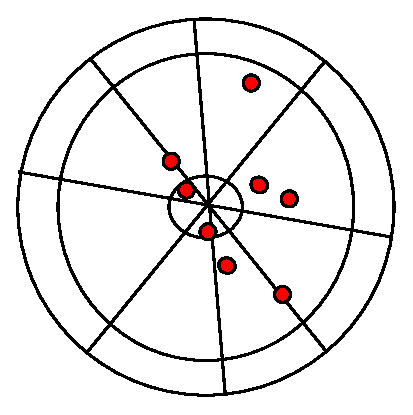
\includegraphics[scale=0.5]{Lab2_figs/bullseye_few.eps}
\end{center}

We now know that this is fairly accurate, but not very precise. We say that
there is a large uncertainty, but that we are aimed about the right
direction. We could get a better estimate of how accurate we are by
repeating the experiment many times:

\begin{center}
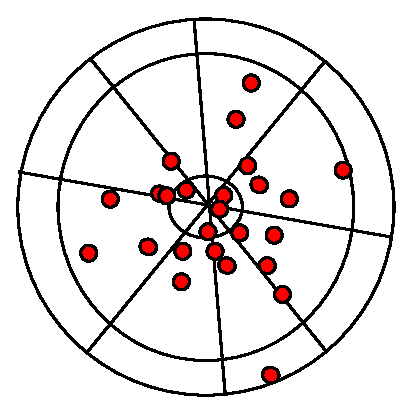
\includegraphics[scale=0.5]{Lab2_figs/bullseye_many.eps}
\end{center}

and finding an average location of the darts:

\begin{center}
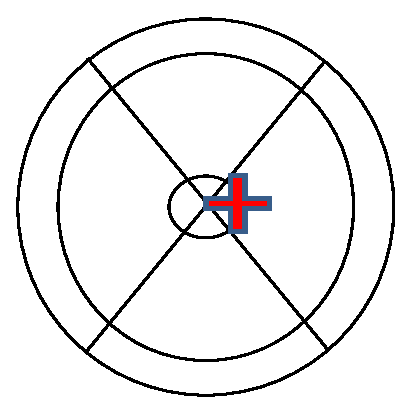
\includegraphics[scale=0.5]{Lab2_figs/bullseye_avg.eps}
\end{center}

This average seems to be just a little right of center. Now we know that we should point the darts a little
to the left. Many experiments are like this. We can repeat the experiment
many times. The uncertainty might be larger than we want, but if we average
over many trials of the experiment, we can find an average value that
represents the actual value of the quantity we are trying to find.

\section{Mean value as our best estimate value}

The mathematical process we use to find the mean is simple and you are
probably quite familiar with it. We simply add up all the values, and divide
the sum by the number of values.%
\begin{eqnarray*}
\bar{x} &=&\frac{x_{1}+x_{2}+x_{3}+\cdots x_{N}}{N} \\
&=&\frac{1}{N}\sum_{i=1}^{N}x_{i}
\end{eqnarray*}%
The last equation uses sigma notation. It is read as \textquotedblleft one
over $N$ times the sum of $x_{i}$ for $i=1$ to $N.$ It is a short-hand
notation for the line above. We will use this notation because it makes
writing our equations much easier. But that means it is very important that
we understand what it means. So let's imagine that we have many values for
the $x$-position for our darts.%
\[
\begin{aligned}
x_{1}&=1.00\pm 0.01\text{cm} \\
x_{2}&=0.50\pm 0.01\text{cm} \\
x_{3}&=-0.75\pm 0.01\text{cm} \\
x_{4}&=-2.25\pm 0.01\text{cm} \\
x_{5}&=3.00\pm 0.01\text{cm} \\
x_{6}&=-0.80\pm 0.01\text{cm} \\
x_{7}&=2.10\pm 0.01\text{cm} \\
x_{8}&=1.2\pm 0.01\text{cm}%
\end{aligned}%
\]%
We have labeled each $x$ with a number. That is what the $x_{i}$ means. The
\textquotedblleft $i$\textquotedblright\ is an index. It stands for any
number from $1$ to $N.$ Our sigma notation says we add up all these
positions, and divide by $N=8$ since there are eight positions%
\begin{eqnarray*}
\bar{x} &=&\frac{\left( 1.00+0.50-0.75-2.25+3.00-0.80+2.10+1.2\right) \text{%
cm}}{8} \\
&=&0.5\text{cm}
\end{eqnarray*}%
which is a little bit to the right of our zero point.

\section{Standard deviation as an estimate of our uncertainty}

But what is our uncertainty? Each of our position measurements were good to $%
\pm 0.01\text{cm}.$ But this can't be what governs our uncertainty. We can
see our points are spread out much more than $\pm 0.01\text{cm}.$ Something
in the experiment (the bad dart thrower) is increasing the uncertainty. We
could use our algebraic method to find the uncertainty, but that would be
tedious and may not include the effects of the dart thrower. It would be
great to have a way to use the spread of the points, itself, to obtain a
numerical estimate of the uncertainty. The spread must include the effects
of the dart thrower.

From your study of statistics, you can guess what we will use to represent
uncertainty, but let's reason it out here. We could take how far each point
is from where we aimed as an indication of how imprecise our throw was. That
would be
\[
\Delta x_{i}=\bar{x}-x_{i}
\]%
for each throw. In this equation we are using the Greek $\Delta $ to show a
difference, and a bar over the $x$ to mean \textquotedblleft the average
value of the $x$-position.\textquotedblright\ Then $\Delta x_{i}$ is how far
off the $i^{th}$ trow from the mean. Sometimes we are off to the right, and
sometimes to the left. If we add up all the $\Delta x_{i}$ values and
average them, they will average to nearly zero most of the time. We can see
that zero is not a good estimate of our uncertainty! So the average
deviation won't work as a measure of uncertainty.

But we can play a trick. The quantity
\[
\Delta x_{i}^{2}=\left( \bar{x}-x_{i}\right) ^{2}
\]%
is always positive. If we averaged $\Delta x_{i}^{2},$
\[
\overline{\Delta x_{i}^{2}}=\frac{1}{N}\sum_{i=1}^{N}\Delta x_{i}^{2}=\frac{1%
}{N}\sum_{i=1}^{N}\left( \bar{x}-x_{i}\right) ^{2}
\]%
nothing would cancel out. And we have solved our calcelation problem. But we
have created another problem by doing this, $\overline{\Delta x_{i}^{2}}$ is
like the square of our how far we are off. So let's take a square root%
\[
\sqrt{\overline{\Delta x_{i}^{2}}}=\sqrt{\frac{1}{N}\sum_{i=1}^{N}\Delta
x_{i}^{2}}=\sqrt{\frac{1}{N}\sum_{i=1}^{N}\left( \bar{x}-x_{i}\right) ^{2}}
\]%
The quantity $\sqrt{\overline{\Delta x_{i}^{2}}},$ represents about how far
off we are on average, it does not tend to zero, and has the same units as $%
x_{i}$ so it can be an estimate of our uncertainty. It is about how far most
of the points are off from the mean. But $\sqrt{\overline{\Delta x_{i}^{2}}}$
is a little hard to write, so we usually give this quantity the symbol $%
\sigma $, which is a Greek letter $s$ and is pronounced \textquotedblleft
sigma.\textquotedblright\ We also give $\sigma $ a name. We call it the
\emph{standard deviation} because it is about how much the average point
\textquotedblleft deviates\textquotedblright\ from the mean position. So for
our $x$-position we can write
\[
\sigma _{x}=\sqrt{\sum_{i=1}^{N}\frac{\left( x_{i}-\bar{x}\right) ^{2}}{N}}
\]%
But what does this math symbology mean? To find $\sigma _{x},$ we must first
find the average positions to find $\bar{x},$ then we take each $x$-position
$\left( x_{i}\right) $ and we subtract the mean from it $\left( x_{i}-\bar{x}%
\right) .$ We square the result. We do this for each of our $x$-positions.
Then we have $\left( x_{1}-\bar{x}\right) ^{2},$ $\left( x_{2}-\bar{x}%
\right) ^{2},$ $\left( x_{3}-\bar{x}\right) ^{2},\cdots \left( x_{N}-\bar{x}%
\right) ^{2}.$ We add these up, and divide by $N$ to find the average $%
\sum_{i=1}^{N}\frac{\left( x_{i}-\bar{x}\right) ^{2}}{N}.$ Then we take the
square root.

In lab today, I\ will ask you to do this by hand once. That should be enough
to convince you that you never want to do it by hand again! Normally we will
use a computer to do this. I suggest you use one of our spreadsheet
programs, or python to do these calculations, and not your calculator.

\section{Histograms}

Suppose I\ plot the results of many, many dart throws. The way I want to
plot this is something you have seen from grading for many years. I want the
horizontal axis to show the $x$-position of the dart throws. I want the $y$%
-axis to show the number of darts that landed at a particular $x$-position.
This type of graph is called a histogram. You often see grades given like
this

\begin{center}
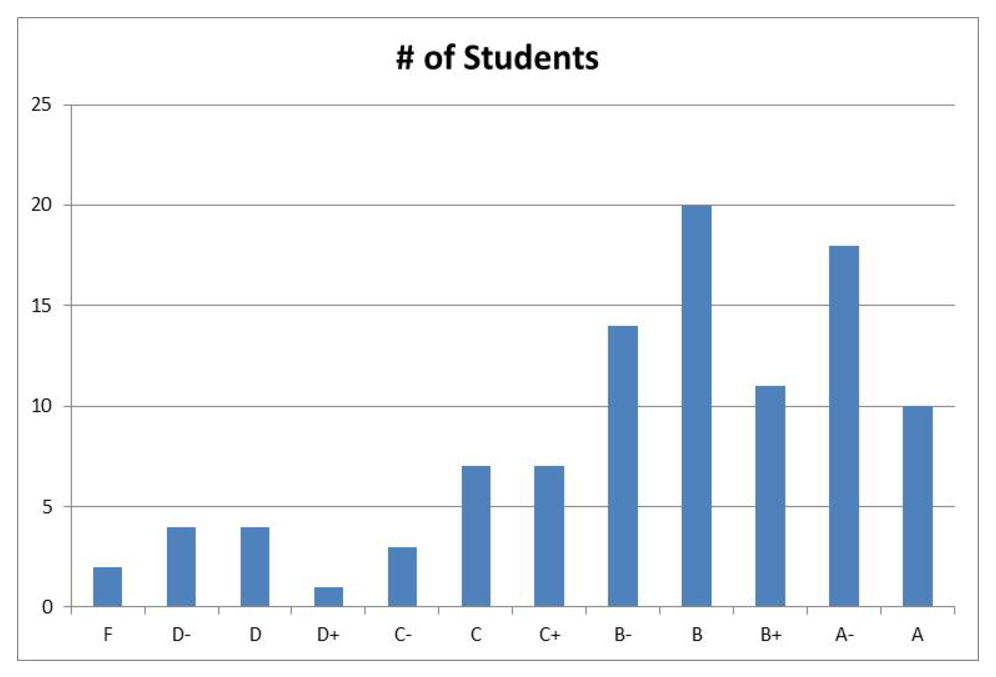
\includegraphics[scale=0.5]{Lab2_figs/hist_few.eps}
\end{center}

where we understand that the bars
indicate how many students got an $A$ (two in this case) and how many got an
$A-$ (five in this case) etc.

If there are many students we can plot their scores and the shape of the
histogram begins to smooth out some

\begin{center}
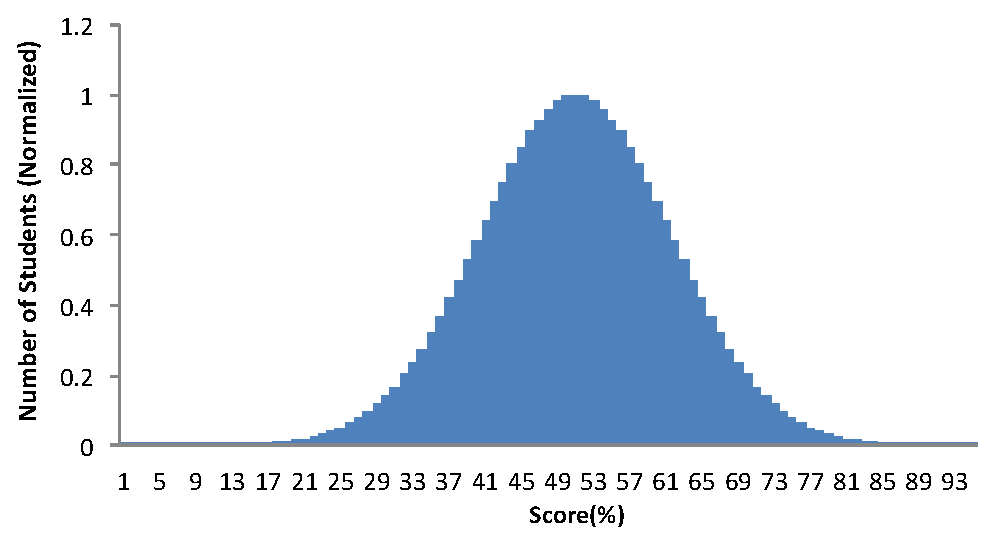
\includegraphics[scale=0.5]{Lab2_figs/hist_many.eps}
\end{center}

If we had infinitely many students, we would get a perfectly smooth curve.
You can see already that coloring in the bars in the graph is not useful any
more. So usually we just draw a point for the top of each bar. These points
form a curve.

\begin{center}
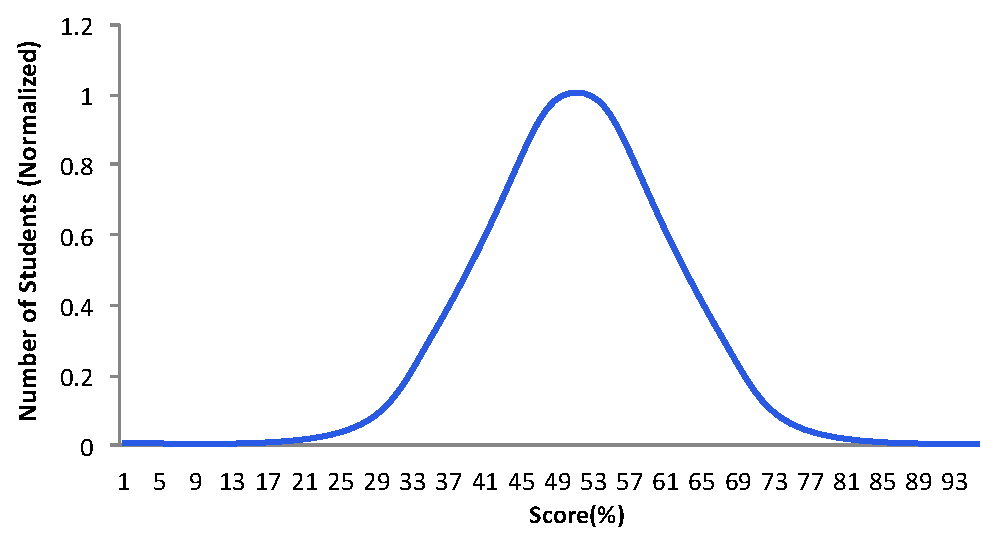
\includegraphics[scale=0.5]{Lab2_figs/hist_smooth.eps}
\end{center}

Unlike student scores, dart positions can be negative. So our dart
distribution should be centered on zero displacement. We will usually find
that $68\%$ of the darts will fall within $\pm \sigma $ of the mean.

\begin{center}
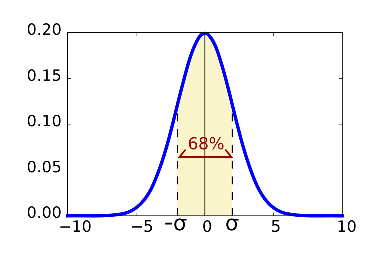
\includegraphics[scale=1.3]{Lab2_figs/normal_68.eps}
\end{center}

We can see that our $\sigma $ value is very like an uncertainty. But there
is a difference. We still have $32\%$ of our experiments outside of $\pm
\sigma ,$ and if we give the uncertainty, $\delta x,$ then all of the
measurements should be within $\pm \delta x.$ If you are building a space
shuttle and absolutely need to guarantee that your error on your calcuation
is within some limit, then you should use a true absolute uncertainty, $\pm
\delta x.$ But for most experiments, being that certain about our
uncertainty is not required, and we can use $\pm \sigma $ as a good
approximation to the uncertainty. We will often do this in this class. If
losing $32\%$ is not acceptable, but finding the true $\delta x$ is not
practical, it is often good enough to use $2\sigma $ or $3\sigma $ as the
estimate of our uncertainty. $95\%$ of the data will fall with $\pm 2\sigma
, $ and $99.7\%$ of the data will fall within $\pm 3\sigma .$ So these are
more conservative estimates than using a single standard deviation. But in
this class we will stick with just $\sigma .$

\section{Standard deviation of the mean}

Now you may wonder, does the mean value get better as we take more
measurements? That is, do we become more sure about where we are pointing if
we throw more darts and include these many darts' locations in our average?
I think you will see from our previous reasoning that this is the case. The
more trials of an experiment that we take, the closer our mean value is to
the \textquotedblleft truth\textquotedblright\ value we are measuring. Since
this is the case, shouldn't the uncertainty go down as we perform more
trials?

The answer is yes. We won't derive this in our class. But the estimate of
the uncertainty should be given by
\[
\sigma _{\bar{x}}=\frac{\sigma _{x}}{\sqrt{N}}
\]%
where $\sigma _{x}$ is our standard deviation in our $x$-position values and
$N$ is the number of trials we took. The more trials that go into our
average, the lower our uncertainty estimate. The value $\sigma _{\bar{x}}$
is called the \emph{standard deviation of the mean}.

Notice that in some of our grade graphs, the most common score was not a $C.$
Here is an example:

\begin{center}
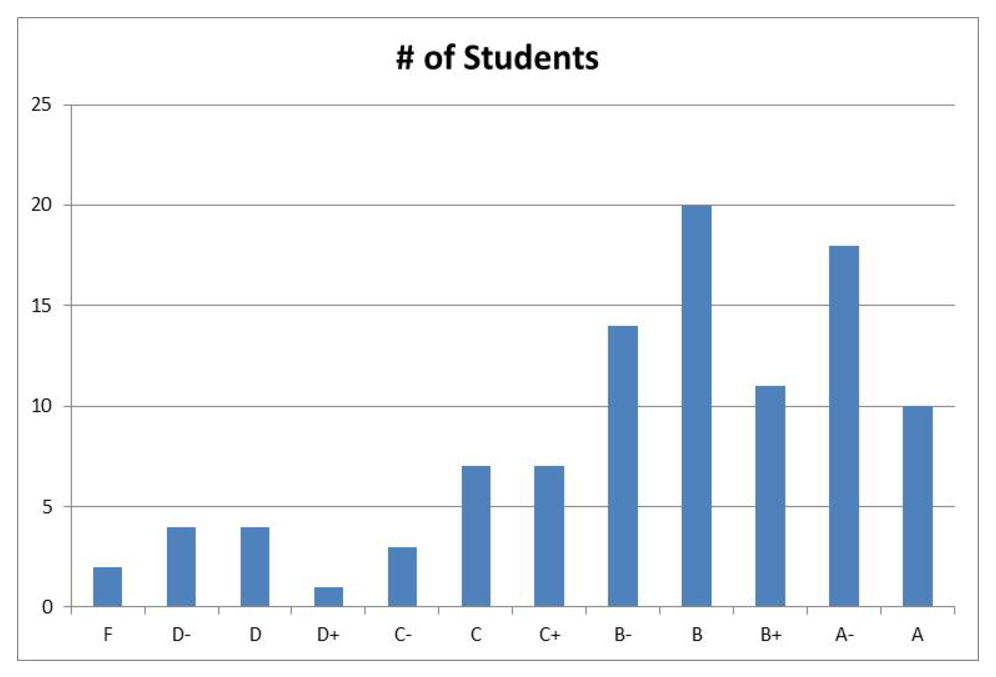
\includegraphics[scale=0.5]{Lab2_figs/hist_few.eps}
\end{center}

As students, this makes us all
happier, but for our error analysis this causes a problem. The error
analysis we have talked about so far assumes that our errors are distributed
in a very uniform way. If I go back to this graph

\begin{center}
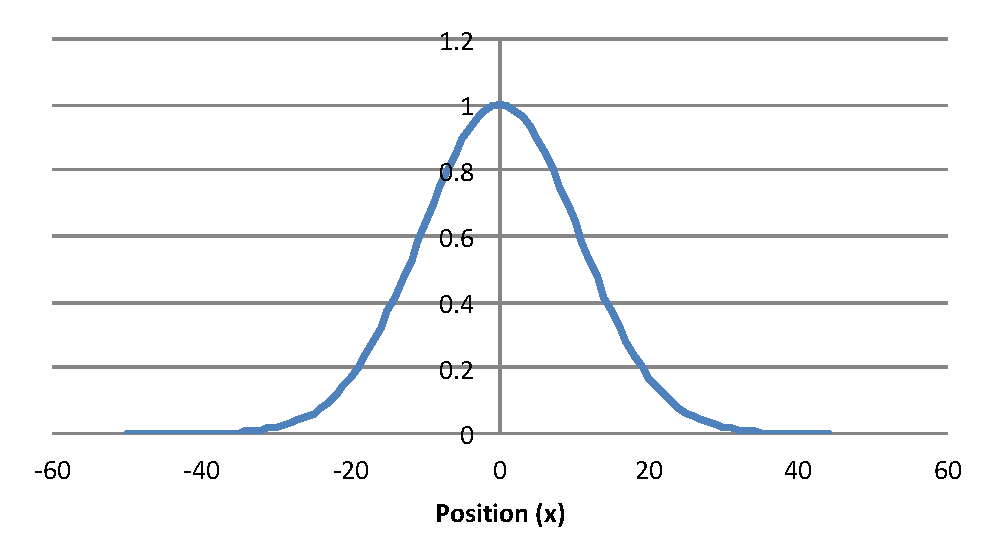
\includegraphics[scale=0.5]{Lab2_figs/hist_dart.eps}
\end{center}

we can see that there are as many
darts that landed to the left as there are to the right. This distribution
of errors is called the \emph{normal distribution}. Usually our errors in
our labs will be normally distributed. That makes all the math we talked
about work. But what if they are not, like our grade example? Well, that is
a great topic for PH336. So for now we will just assume a normal
distribution. But we can check to see how non-normal our data is. We can
find the \emph{mode} which is the value that occurs most frequently. For our
grade distribution above it would be a $B.$

We can also find the place where half of the trials landed on one side and
half on the other. This is called the \emph{median} point. We will calculate
both in our lab today. If we have a normal distribution, the average,
median, and the mode will all be the same. If this is not the case, then we
may worry a little about our error estimate--it may be too small.

\section{Graphical reporting of the mean (expected value) and standard
deviation (uncertainty)}

We now have a new view of measurement based on statistics. The mean value is
the value that we will say is our measurement. We call this the \emph{%
expected value}. The standard deviation is the representation of our
uncertainty. We can plot this in a way that communicates both at once. If we
take our eight data points that we started with earlier, we know the mean , $%
0.5\text{cm},$ and we can find the standard deviation of the mean to be $0.6%
\text{cm}.$ We plot this by making a dot or diamond or some larger point
indicator. Then we make a line through the point with little ends that show
the size of the uncertainty. The result looks like this.

\begin{center}
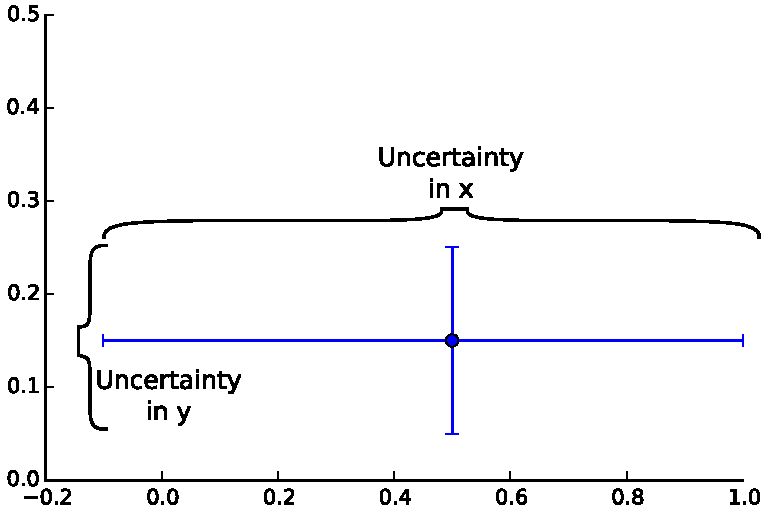
\includegraphics[scale=0.6]{Lab2_figs/error_bars.pdf}
\end{center}

 Excel, and most plotting programs will allow you to
add error bars to your graphs.

Of course, we could have $y$
-direction error bars as well. These would be vertical, and there is no reason the $y$%
-error would be the same as the $x$-error. We may encounter such situations
in future labs.

\end{document}

\documentclass[twoside,11pt,ShortChapTitles]{BYUTextbook}

\usepackage{soul}
\renewcommand{\vec}[1]{\ensuremath{\mathbf{#1}}}
\usepackage{siunitx}
\sisetup{round-mode = figures,
  round-precision = 3, scientific-notation=true}
  \usepackage{marginfix}

\usepackage{mathtools}

%\lstMakeShortInline[columns=fixed]|


\setcounter{chapter}{2}

\begin{document}

\chapter{Measurement and Uncertainty II}
\section*{Python You Should Know for This Chapter}
\begin{itemize}
\item What these terms mean, and how to work with them: {\em string, int, float}
\item How to import the \code{matplotlib} plotting library and its basic plotting commands.
\end{itemize}
Recommended reading: Introduction to Scientific Computing in Python, by Nelson and Zachreson; All of chapter 7, Basic Plotting
\section*{Questions that you should be able to answer by the end of this chapter.}
\begin{enumerate}
\item What is $\frac{\partial}{\partial x} \frac{x^2}{yz}$?
\item What is $\frac{\partial}{\partial t} \frac{5}{t^2}$?
\item You want to find out how many moles, $N$, of an ideal gas are in a container.  You can measure its volume, $V$, temperature, $T$, and pressure, $P$.  You also know that those quantities are related to the number of moles through the ideal gas law:
\[PV=NRT\]
where $R$ is the universal gas constant and has negligible uncertainty.  Write out a symbolic equation to calculate the number of moles of gas in the container and a separate equation for the uncertainty in your calculation.
\end{enumerate}
\hrulefill


By now, you should be far enough in your calculus class to know what a derivative is.  If not, the most important thing you need to know is that it's a mathematical method to calculate the slope of any function at any point on that function.

\section{The Power Rule}
The most commonly used derivative rule\sidenote{Derivatives actually have several different rules that you can memorize: chain rule, quotient rule, trig rules, and many more that you will learn (or should have learned) in your calculus class. Every single one of them comes from taking the limit of $\frac{y_2-y_1}{x_2-x_1}$ as the distance between $x_1$ and $x_2$ goes to zero.} is the power rule\sidenote{Most of what we do in this class will use the power rule, just ask for help if you run into something odd like an $\arctan$ function.}:

\[
\frac{d}{dx}\left(  ax^{n}\right)  =anx^{n-1}
\]
that is, if I have a constant, $a,$ times $x^{n}$ the slope of this curve is
the constant, $a,$ times the power, $n,$ times $x$ to the $n-1$ power.

Let's take an example. What is the slope of the function $y=5x^{3}?$

\[
\frac{d}{dx}\left(  5x^{3}\right)  =\left(  5\right)  \left(  3\right)
x^{3-1}=15x^{2}
\]


How about finding the slope of $y=7x^{2}-2x+1$\sidenote{Notice how you can handle each additive term separately.}

\[
\frac{d}{dx}\left(  7x^{2}-2x+1\right)  =\left(  7\right)  \left(  2\right)
x^{1}-\left(  2\right)  (1)x^{0}+0
\]

The last term illustrates that the slope of a constant is zero. That makes
sense. Constants don't change. So the change in $y$ just due to the last term
$(1)$ should be zero. We also remember $x^{0}=1.$ So we are left with
\[
\frac{d}{dx}\left(  7x^{2}-2x+1\right)  =14x-2
\]


There are many functions where you can use the power rule, but where it is not readily apparent.  For example, when $x$ is in the denominator\sidenote{Remember that $1/x^n = x^{-n}$}:
\[ \frac{d}{dx}\frac{5}{x^3} = \frac{d}{dx} 5x^{-3} = (-3)*5x^{-4} = -\frac{15}{x^4}\]
or square roots:

\[
\frac{d}{dx}\left(  \sqrt{x}\right)  =\frac{d}{dx}\left(x^{\frac{1}{2}}\right)  =\frac{1}{2}x^{-\frac{1}{2}} = \frac{1}{2}\frac{1}{\sqrt{x}}
\]


\section{How Derivatives Relate to Uncertainty}
In Lab 1, we discussed Standard Error Propagation\sidenote{If you used the algebraic error propagation methods, you should go back and read the Standard Error Propagation section of that Lab.} and how you needed to find partial derivatives\sidenote{Remember: a partial derivative is just a regular derivative where you treat anything except the variable that you are taking the derivative with respect to as a constant.  For example, \[\frac{\partial}{\partial x} y^3x^2 = 2y^3x\]
and \[\frac{\partial}{\partial y} y^3x^2 = 3y^2x^2\]
We use $\partial$ instead of $d$ to denote a partial derivative.} in order to calculate the uncertainty in our calculated values.

Here's an example of why.  Suppose you shoot a ball up into the air and want to predict how high it will be $0.15$ seconds after you shoot it.  Kinematics predicts that the ball's $y$ postion vs. time graph should look like this
\begin{center}
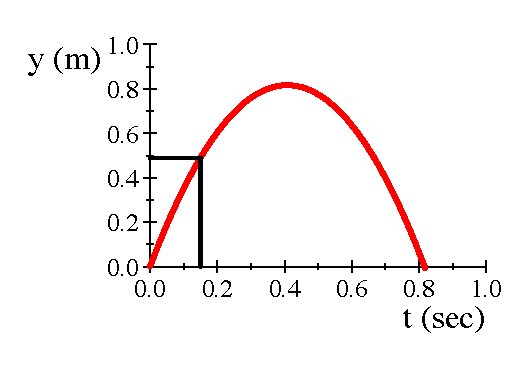
\includegraphics{Lab3_figs/Parab_onepoint.eps}
\end{center}
and that the ball should be at a height of 0.5 meters after 0.15 seconds.  However, with the stopwatch we use, the best measurement we can get is $0.15 \pm 0.05$ seconds.  Adding the time uncertainty to the graph
\begin{center}
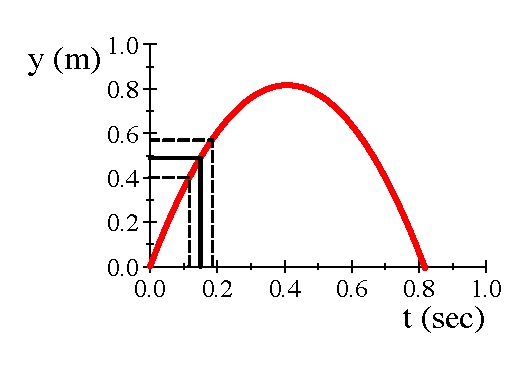
\includegraphics{Lab3_figs/Parab_threepoints.eps}
\end{center}
shows that our predicted height could be anywhere from 0.4 m to 0.6 m.

Notice that the line segment between our two dotted lines is roughly linear, and we could approximate it with this equation\sidenote{Note: $\left.\frac{\partial y}{\partial t}\right|_{t=t_0}$ is the mathematical way to write: the derivative of our function $y$ with respect to $t$ evaluated at $t_0$.}:
\[y = \left.\frac{\partial y}{\partial t}\right|_{t=t_0}t+b = m_{t_0}t+b\]
where $\left.\frac{\partial y}{\partial t}\right|_{t=t_0} = m_{t_0}$ and represents the slope of our line at $t_0=0.15$ seconds (where it is crossed by the solid black line).

With a little bit of algebra, we can use this equation to estimate how far away the value at our high point ($y_h$, where $t_h=0.2$ seconds) would be from our calculated point, $y_h$:

\begin{tabular}{rcc}
$y_h =$& $m_{t_0}t_h$ &$+b$ \\
$=$& $m_{t_0}\left(t_0+\delta t\right) $&$ + b$\\
$=$& $m_{t_0}\delta t$ & $m_{t_0}t_0 + b$\\
$=$& $\delta y$ & $+ y_0$
\end{tabular}

\noindent This equation shows us that our uncertainty in $y$ is our slope at our mean value in $t$ ($m_{t_0}$), multiplied by our uncertainty in time, $\delta t$.

Using $\delta y = m_{t_0}\delta t$ is roughly equivalent to using the high/low method from Lab 1. Using a high/low method assumes that any time between 0.1 and 0.2 seconds is equally likely.

But in Lab 2, you learned about normal (also called Gaussian) distributions (see Fig. \ref{Lab2_figs/normal_68.eps}
\marginfig{Lab2_figs/normal_68.eps}{A normal distribution. The region within one standard deviation of the mean is highlighted.}
and saw that if a measured time is $0.15 \pm 0.05$ seconds, you are more likely to measure a time of 0.16 seconds than you are to measure a time of 0.2 seconds.

The rules for standard error propagation\sidenote{Standard error propagation also assumes that your measurements are independent, e.g. how you measure time with a stop watch does not affect how you measured distance with a meter stick.  It is generally a safe assumption to make.} use a statistical principle called the {\em central limit theorem} to take this variance in probability into account.  This derivation is beyond the scope of this lab manual, but the result is the equation from Lab 1:
 \[
 \left(\delta f(x,y,z,....)\right)^2 = \left(\frac{\partial f}{\partial x}\right)^2(\delta x)^2+ \left(\frac{\partial f}{\partial y}\right)^2(\delta y)^2++ \left(\frac{\partial f}{\partial z}\right)^2(\delta z)^2+...
 \]
Which you will often see written in summation notation:
\[
\delta f=\sqrt{\sum_{i=1}^{N}\left(  \frac{\partial f}{\partial x_{i}}\right)
^{2}\delta x_{i}^{2}}
\]




\end{document}

%==================Old Material, archived ===============================================
I\ hope that by now you have been taught what a derivative is in your Math 112
class. But if not, we will learn what it is today. For our purposes, a
derivative is a slope of a line. You should recognize the equation of a
straight line as
\[
y=mx+b
\]
The slope $m$ can be written as
\[
m=\frac{dy}{dx}
\]
This is nothing magic. It is just a strange way to write $m.$ With the slope
written this way, the equation of the line could be written as
\[
y=\frac{dy}{dx}x+b
\]
But why $dy/dx$? Think of how we find a slope of a line. Back in junior high
school we called the slope the  ``rise over
run.'' That is, the change in $y$-value divided by the change
in the $x$-value.
\[
m=\frac{y_{2}-y_{2}}{x_{2}-x_{1}}
\]
In physics, we write the change in a variable using the greek letter delta,
$\Delta.$ So we could write the slope as
\[
m=\frac{y_{2}-y_{2}}{x_{2}-x_{1}}=\frac{\Delta y}{\Delta x}
\]
\ We need to get used to this delta notation, so let me write out $\Delta y$
\[
\Delta y=y_{2}-y_{1}
\]
and $\Delta x.$
\[
\Delta x=x_{2}-x_{1}
\]
So our straight line equation should be written
\[
y=\frac{\Delta y}{\Delta x}x+b
\]
but if we take $\Delta x$ to be very, very small it is customary to write the
$\Delta x$ as just $dx$ (I guess a  ``d'' is
smaller than a  ``$\Delta$"). If this is not
familiar from Math 112, is should be by now from PH121 (if is not familiar at
all, call me over for help, but still don't panic--we are just writing slope
in a strange way).

In PH121 you have or will shortly learn that the velocity is the slope of the
plot of $x$ vs. $t,$ for example,
\[
y=\frac{1}{2}\frac{\text{m}}{\text{s}}t+1\text{m}
\]
is an equation giving the $y$ position of an object as a function of time.
Note that it is a straight line on a $y$ vs. $t$ plot.
\begin{center}
\hspace*{-1.5cm}
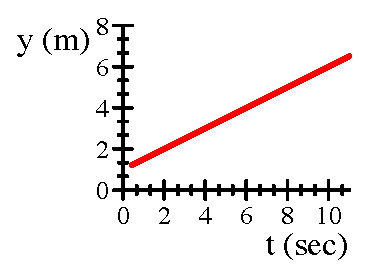
\includegraphics{Lab3_figs/LineGraph.eps}
\end{center}
The slope of the line is
\[
\frac{dy}{dt}=\frac{1
\text{m}
}{2
\text{s}
}
\]
We can verify that this works by looking at the plot and noting that for every
two units of time, we go up one position unit. The slope is $1/2\frac{
\text{m}
}{
\text{s}
}.$

But not all curves are straight lines. What do we do with curves that, well, curve?

One idea is that we could split up the curve into little line segments, each
with its own slope. We can think of $dy/dt$ as an instantaneous slope, a slope
of one of the tiny line segments that make up our curve. This is the sort of
speed measurement that your speedometer gives. The speed might be different a
short time later. But right now the speed is, say, $0.5
\text{m}
/
\text{s}
.$

\begin{center}
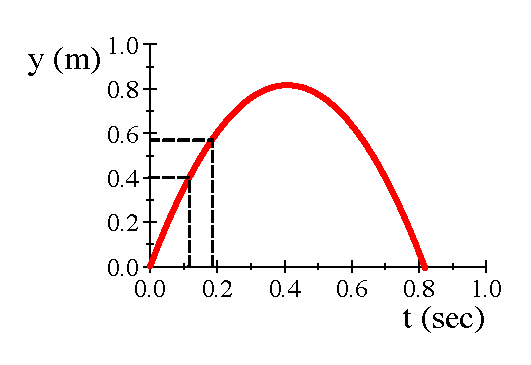
\includegraphics{Lab3_Figs/Parab_twopoints.eps}
\end{center}
Really, in defining an instantaneous slope we have assumed that the slope near
our point on the curve is essentially a straight line if $\Delta t$ is small enough.

We can use this idea to interpret our error calculations. Suppose I\ throw a
ball in the air with a initial speed of $4
\text{m}
/
\text{s}
$ straight up starting from $y_{o}=0$. From PH121 you have learned (or will
soon learn) that the equation for predicting how high the ball will go is
\[
y=y_{o}+v_{o}t+\frac{1}{2}at^{2}
\]
It says that starting at $y_{o}$ the ball will go higher depending on the
initial velocity, $v_{o},$ and the acceleration, $a.$ That make sense.

At a time, $t,$ the ball should be at
\[
y=0+4\frac{
\text{m}
}{
\text{s}
}t-\frac{1}{2}\left(  9.8\frac{
\text{m}
}{
\text{s}
^{2}}\right)  t^{2}
\]
where $a=-9.8\frac{
\text{m}
}{
\text{s}
^{2}}$ is the acceleration due to gravity. So, knowing this, I could predict
how high the ball would go if I\ pick a particular time, say, $0.15
\text{s}
.$ The result should be
\begin{align*}
y  & =0+4\frac{
\text{m}
}{
\text{s}
}\left(  0.15
\text{s}
\right)  -\frac{1}{2}\left(  9.8\frac{
\text{m}
}{
\text{s}
^{2}}\right)  \left(  0.15
\text{s}
\right)  ^{2}\\
& =0.489\,75
\text{m}
\end{align*}
This is shown in the next figure with a black line. Solving the equation for
$y$ is equivalent to drawing a line up to the curve, then from our spot on the
curve over to the $y$-axis to find the position.
\begin{center}
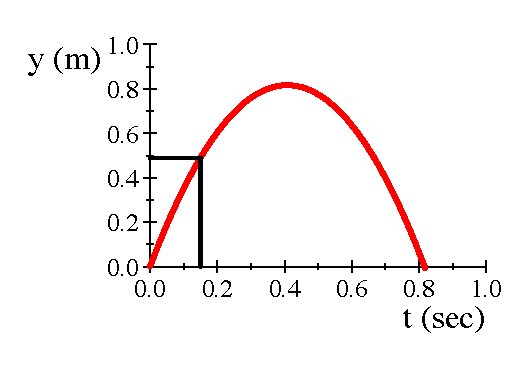
\includegraphics{Lab3_figs/Parab_onepoint.eps}
\end{center}


For our case we plot a line upward from $0.15
\text{s}
$ to the curve, and then plot a horizontal line from the intersection to the
$y$-axis. We can see that we get $4.9
\text{m}
.$ Suppose I try to verify this by taking a picture of the ball in flight at
$0.015
\text{s}
,$ but my stop watch is only good to $\pm0.005$ seconds. I try to take the
picture when the watch is at $0.015
\text{s}
,$ but I might have taken the picture at $0.01
\text{s}
$ or at $0.02
\text{s}
$ or anywhere in between. My time has some uncertainty. What does the
uncertainty in my stop watch time mean for the uncertainty in my $y$ value?

We can get a good approximation by graphically drawing vertical lines up from
$t_{\min}$ and $t_{\max}$ to the curve, and then extending horizontal lines
from the intersections to the $y$-axis. This gives us a $y_{\min}$ and
$y_{\max}.$ Our actual height could be anywhere in between these. This is a
way to view our uncertainty in $y.$
\begin{center}
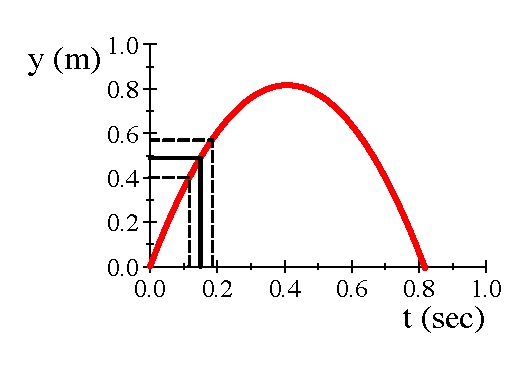
\includegraphics{Lab3_Figs/Parab_threepoints.eps}
\end{center}


We can use this idea to find a general way to calculate uncertainties. We
could define $\Delta t=t_{\max}-t_{\min}$. If our $\Delta t$ is small enough
(so we can write it just $dt$), the curve is essentially a straight line in
the region between $t_{\min}$ and $t_{\max}.$ So if we knew the slope of that
line (the derivative $dy/dt$) we could easily figure out the $y_{\max}$ and
$y_{\min}$ points to get our uncertainty range, at least if we stay near our
$t_{n}$ part of the curve. Recall that our uncertainty in $y $ using the
high/low method is
\[
\delta y=\frac{y_{\max}-y_{\min}}{2}=\frac{\Delta y}{2}
\]
Remembering that
\[
y=\frac{dy}{dt}t+b
\]
then
\begin{align*}
\Delta y  & =y_{\max}-y_{\min}\\
& =\frac{dy}{dt}t_{\max}+b-\frac{dy}{dt}t_{\min}-b\\
& =\frac{dy}{dt}\Delta t
\end{align*}
From your reading, you will recognize this as almost the uncertainty in a
function of one variable! But even if you don't recognize it, we can show that
this is true using our high/low method. The quantity $\Delta t$ is
\[
\Delta t=t_{\max}-t_{\min}
\]
so our uncertainty in $t$ would be
\[
\delta t=\frac{t_{\max}-t_{\min}}{2}=\frac{\Delta t}{2}
\]
then
\begin{align*}
\delta y  & =\frac{y_{\max}-y_{\min}}{2}\\
& =\frac{1}{2}\frac{dy}{dt}\Delta t\\
& =\frac{dy}{dt}\frac{\Delta t}{2}\\
& =\frac{dy}{dt}\delta t
\end{align*}
so
\[
\delta y=\frac{dy}{dt}\delta t
\]
So our uncertainty in $y$ is just the slope at our point on the curve
multiplied by our uncertainty in $t.$

But what if we have more than one variable? Say, we have a function $y(x,z),$
we essentially have a two dimensional slope. Think of a hill, you can go down
a hill in more than one direction. So we need slope parts for each direction
we can go.

But there is a fix we need to make to this equation that you won't learn for
several math classes to come. We want to have a slope in the $x$ and $z$
direction, but we want the slopes to be independent (if you have already taken
PH121, think of two dimensional motion problems, we split the problem into
components). The notation for this is
\[
\Delta y=\frac{\partial y}{\partial x}x+\frac{\partial y}{\partial z}z
\]
where
\[
\frac{\partial y}{\partial x}
\]
means the component of the slope just in the $x$ direction. We take a
derivative of the function $y,$ but assume only $x$ is a variable (treat $z$
and all $z$ terms with no $x^{\prime}s$ as constants). This lets us separate
the $x$ and $z$ parts. A special, one variable derivative like $\partial
y/\partial x$ is called a \emph{partial derivative} because you only take one
dimension of the derivative at a time. The reading from Chapter 3 uses this
type of derivative to find the general formula for error propagation. If we
wish to find the error in some general function $z\left(  x,y\right)  $ the
error is given by
\[
\delta y=\sqrt{\left(  \frac{\partial y}{\partial x}\right)  ^{2}\delta
x^{2}+\left(  \frac{\partial y}{\partial z}\right)  ^{2}\delta z^{2}}
\]
This looks a lot like our slope equation What we are doing is to assume the
function $y\left(  x,z\right)  $ is flat in a small region around the point we
are studying. then the function has a slope $\partial y/\partial x$ in the $x
$-direction, and $\partial y/\partial z$ in the $y$-direction. Each term like
\[
\left(  \frac{\partial y}{\partial x}\right)  \delta x
\]
gives how far off we could be in that direction (the $x$-direction in this
case). Remember that we have assumed that $y\left(  x,z\right)  $ is
essentially flat near our point of interest. The square root may be something
of a mystery, but remember what you have learned or are learning about adding
vectors in PH121. We add components of a vector to find the magnitude like
this
\[
V=\sqrt{V_{x}^{2}+V_{y}^{2}}
\]
This comes from the Pythagorean theorem. The $x$ and $y$ parts of the vector
form two sides of a triangle. We want the remaining side. So we use the
Pythagorean theorem to find the length of the remaining side.

We are doing the same for our small uncertainty lengths. We are just adding
the $x$ and the $y$ components of the error. We could write our error formula
for the general case of a function $f$, that depends on $N$ different
variables.
\[
\delta f=\sqrt{\sum_{i=1}^{N}\left(  \frac{\partial f}{\partial x_{i}}\right)
^{2}\delta x_{i}^{2}}
\]
We will use this formula a lot, so make sure you understand what it means (ask
your instructor for help if it is not clear).

\section{How do we find the slope?}


\section{Tie to statistics}

We need to tie our statistical ideas into what we have learned about error
propagation. Lets go back to our function $f\left(  x,y\right)  $ the error is
given by
\[
\delta f=\sqrt{\left(  \frac{\partial f}{\partial x}\right)  ^{2}\delta
x^{2}+\left(  \frac{\partial f}{\partial z}\right)  ^{2}\delta z^{2}}
\]
but now we know we could express this in terms of standard deviations
(provided you don't need to ensure all data are within your uncertainty
range). We can write our uncertainties as
\[
\sigma_{f}=\sqrt{\left(  \frac{\partial f}{\partial x}\right)  ^{2}\sigma
_{x}^{2}+\left(  \frac{\partial f}{\partial z}\right)  ^{2}\sigma_{z}^{2}}
\]


We can use this to show that the standard deviation of the mean (the best
estimate of our uncertainty) is given by

\[
\sigma_{\bar{x}}=\frac{\sigma_{x}}{\sqrt{N}}
\]
Think of calculating a mean value
\[
\bar{x}=\frac{x_{1}+x_{2}+\cdots x_{N}}{N}
\]
We can find the uncertainty in this function $\sigma_{\bar{x}}$
\[
\sigma_{\bar{x}}=\sqrt{\left(  \frac{\partial\bar{x}}{\partial x_{1}}\right)
^{2}\sigma_{x_{1}}^{2}+\left(  \frac{\partial\bar{x}}{\partial x_{2}}\right)
^{2}\sigma_{x_{2}}^{2}+\cdots+\left(  \frac{\partial\bar{x}}{\partial x_{N}
}\right)  ^{2}\sigma_{x_{N}}^{2}}
\]
You see we just take the partial derivative of our function $\bar{x}$ with
respect to each of the variables $x_{i}$ and multiply by the uncertainty in
that variable written now as a standard deviation $\sigma_{i}.$

For this special case, all of the $x_{i}$ are the same (we are measuring the
same value over and over in taking an average) and all of the $\sigma_{i}$ are
the same so we just have
\[
\sigma_{\bar{x}}=\sqrt{N\left(  \frac{\partial\bar{x}}{\partial x_{1}}\right)
^{2}\sigma_{x_{1}}^{2}}
\]
and we can take the derivative using our rule. Only $x_{1}$ is a variable, so
we can write the average $\bar{x}$ as
\[
\bar{x}=\frac{x_{1}}{N}+\frac{x_{2}+\cdots x_{N}}{N}
\]
This is a polynomial! The first term is $\frac{1}{N}x_{1}$ and the whole
second term is a constant if we take a partial derivitive with respect to
$x_{1}$. The derivative is
\begin{align*}
\frac{\partial\bar{x}}{\partial x_{1}}  & =\frac{\partial}{\partial x_{1}
}\left(  \frac{x_{1}+x_{2}+\cdots x_{N}}{N}\right) \\
& =\frac{1}{N}x_{1}^{0}+0\\
& =\frac{1}{N}
\end{align*}
so our statistical error function is just
\begin{align*}
\sigma_{\bar{x}}  & =\sqrt{N\left(  \frac{1}{N}\right)  ^{2}\sigma_{x_{1}}
^{2}}\\
& =\sqrt{\frac{\sigma_{x_{1}}^{2}}{N}}\\
& =\frac{\sigma_{x_{1}}}{\sqrt{N}}
\end{align*}
or, since all the $\sigma_{x_{i}}$ are the same, we can just write this as
\[
\sigma_{\bar{x}}=\frac{\sigma_{x}}{\sqrt{N}}
\]


Notice that in this example we had many $x_{i}$ and that to find the
uncertainty we just extended our equation from two variables
\[
\sigma_{f}=\sqrt{\left(  \frac{\partial f}{\partial x}\right)  ^{2}\sigma
_{x}^{2}+\left(  \frac{\partial f}{\partial z}\right)  ^{2}\sigma_{z}^{2}}
\]
to $N$ variables
\[
\sigma_{f}=\sqrt{\sum_{i=1}^{N}\left(  \frac{\partial f}{\partial x_{i}
}\right)  ^{2}\sigma_{i}^{2}}
\]


In this special case, we were trying to show a special result, but we can do
this for any function with any number of variables. If your function is
complicated, you just need to take more partial derivative terms under the
square root.


\end{document}

\documentclass[twoside,11pt,ShortChapTitles]{BYUTextbook}

\usepackage{soul}
\renewcommand{\vec}[1]{\ensuremath{\mathbf{#1}}}
\usepackage{siunitx}
\sisetup{round-mode = figures,
  round-precision = 3, scientific-notation=true}
  \usepackage{marginfix}

\usepackage{mathtools}






\setcounter{chapter}{3}

\begin{document}
\chapter[Experimental Design I]{Experimental Design I: Harmonic Oscillators (masses and springs)\label{Experimental Design}}
\section*{Python You Should Know for This Chapter}
\begin{itemize}
\item How to create a user-defined function, as well as pass information to that function and get information back out.
\item How to import user defined functions.
\item How to do math with arrays.
\end{itemize}
Recommended reading: Introduction to Scientific Computing in Python, by Nelson and Zachreson; Section 4.3, all of chapter 5, and if you have time, chapter 12.
\section*{Questions that you should be able to answer by the end of this chapter.}
\begin{enumerate}
\item A mass oscillating up and down on a spring should have a period $T$ of $T=2\pi\sqrt{m/k}$ where $m$ is the mass of the mass and $k$ is the stiffness of the spring.  In your experiment, the dependent variable is $T$, and your independent variable is $m$.  What is the proper linearized version of the period equation?
\item Here is a simple Python function:
\begin{Verbatim}
def switch(a,b):
    return b,a

\end{Verbatim}
How would I use it to switch the values stored in variables \code{x} and \code{y}?
\item Last week you calculated the acceleration due to gravity of a tennis ball by timing how long it took to fall.  How do the experimental design steps in this reading apply to your process?
\end{enumerate}
\hrulefill


\section{Getting better accuracy by fitting data}
In the last lab, we used the mean and standard deviation to find a measurement and its error.  We then used our measurements and error propagation to calculate $g$ and the error in our calculation.

What if you wanted better accuracy?  One option would be to just repeat the same measurement many different times in hopes of getting a better mean value.  However, if the person doing the timing always ends the timer a little too soon, or your scale actually reads 5 kg when it should read zero, repeating the measurement won't help you gain any more accuracy.

But if you change how your measuring a little bit each time, by dropping the ball from a different height, or changing the length of your pendulum string, you can get a better calculated value, even if your measurement technique is off.  \sidenote{As long as it is consistently wrong.  If your scale is 5 grams off when you weight something that is 20 grams, and 50 grams off when you weight something at 100 g, you need a new scale.}

This section will show you how.

\subsection{Linear Least Squares}

Linear least squares is the most common type of data fitting (other than just averaging) because it is fast, easy (once you get the hang of it), and it has a known solution. (It's a plug and chug formula)
Many types of fits just have a computer try a bunch of values and see which one fits the best.  Sometimes the computer will miss the actual best fit for something that is just better than the choices around it, and even if the computer does find the best fit, it will take much longer to get there.

Here is the basics of how least squares fitting works.  Imagine that you've taken the data shown below:

\begin{center}
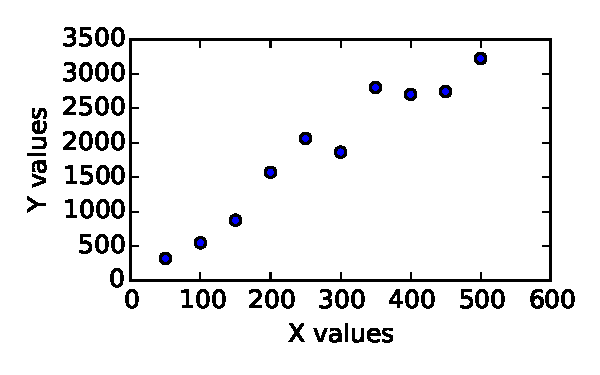
\includegraphics{Lab4_figs/dataScatter.pdf}
\end{center}

The data wiggles all over the place, but it is easy to see that it generally follows a line.  Therefore, we'd predict that our data should match:
\[y=mx+b\]
But there is no single line that will go through every single data point.  There's always a little bit of error, often written as $\chi$, and it represents the little green lines in the figure below:
\begin{center}
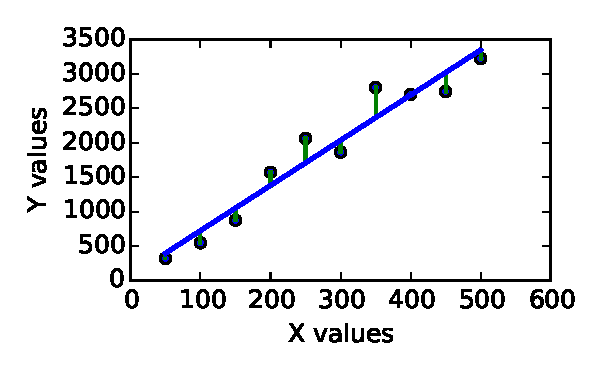
\includegraphics{Lab4_figs/dataWfit.pdf}
\end{center}

My data actually matches this equation:
\[y_i=mx_i+b+\chi_i\]
Where $y_i$ is the $y$ value corresponding to each individual $x$ value, $x_i$.  $\chi_i$ gives how far away each data point is from the line. We can solve for how far away from the line each data point is:
\[\chi_i=y_i-b-mx_i\]
and come up with a function that gives us a total error:
\[E_{tot}=\sum_i^N \chi_i^2 = \sum_i^N (y_i-b-mx_i)^2\]
which is just the sum of how far off every single data point is from the line.  We use $\chi_i^2$ as an easy way to get the absolute value of each error.  We really only care about how far each data point is from the line, not whether it is above or below the line.

Using calculus, we can find the slope and intercept of the line that will minimize the our total error.  To minimize, we just take the derivative of our error function with respect to the thing we want to minimize, and set it equal to zero:
\[\frac{\partial E_{tot}}{\partial m}=0;\,\,\,\frac{\partial E_{tot}}{\partial b}=0\]
If you do those derivatives, and use the two equations to solve for $m$ and $b$, you get this:
\[m=\frac{\left<xy\right>-\left<x\right>\left<y\right>}{\left<x^2\right>-\left<x\right>^2}\]
\[b=\left<y\right>-m\left<x\right>\]
where $m$ and $b$ are the slope and intercept of the line that gets closest to all of the data points.  The $\left<\right>$ symbols mean the average of the thing inside. $\left<x\right>$ is the average of all the $x$s.  To calculate $\left<xy\right>$ you'd multiply each $x$ value by its corresponding $y$ value, then take the average.
Using error propagation, you can find the errors in you fit.  The error in the slope is:
\[\sigma_m=\frac{\sigma_y}{\sqrt{N\left(\left<x^2\right>-\left<x\right>^2\right)}}\]
and the error in the intercept is:
\[\sigma_b=\sigma_y\sqrt{\frac{\left<x^2\right>}{N\left(\left<x^2\right>-\left<x\right>^2\right)}}\]
$\sigma_y$ represents the average error of each y value, and is calculated using:
\[\sigma_y=\sqrt{\frac{1}{N-2}\sum_i^N \left(y_i-b-mx_i\right)^2}\]

For reference, here is a figure with the best fit line for to the data.  The red lines mark the high/low values given by the error in the slope:
\begin{center}
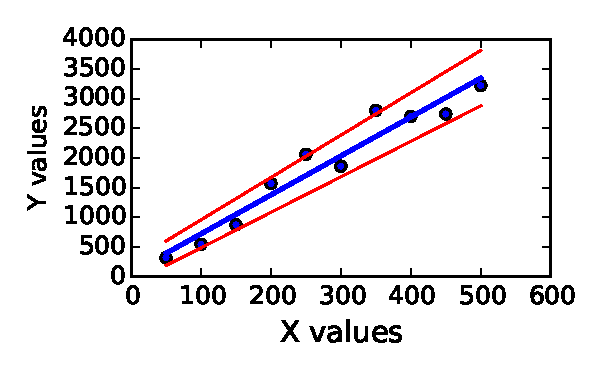
\includegraphics{Lab4_figs/dataWfitRange.pdf}
\end{center}

Here's an example of a Python function that takes in x and y values and returns the slope and intercept of the best fit line\sidenote{It will be up to you to add a part that calculates their errors.}.  It would be very go practice to read through it and see if you can figure out what each line does.
\begin{Verbatim}
def linear_least_squares(x,y):
    #Import numpy
    import numpy as np
    #Get the number of data points
    N=len(x)

    #Make sure x and y are numpy arrays to make array math easy
    x=np.asarray(x)
    y=np.asarray(y)

    #Calculate the average values needed to find the slope and intercept
    xbar=np.mean(x) #Average Value of the xdata
    ybar=np.mean(y) #Average value of the y data
    xbar2=np.mean(x**2) #Average value of the xdata squared
    xybar=np.mean(x*y) #Average value of xdata*ydata



    #Use the linear least squares formula to calculate
    #the slope and the intercept of the best fit line
    slope=(xybar-xbar*ybar)/(xbar2-xbar**2)
    intercept=ybar-slope*xbar

    return slope, intercept

\end{Verbatim}

Once coded, you can use the function like this:
\begin{Verbatim}
x_data = [10,20,30,40,50]
y_data = [20,40,60,80,100]

#Notice that the input/output variable names do not have to match
#what you called them in the function definition.
m,b = linear_least_squares(x_data,y_data)
#Now the slope of my fit is stored in m
#and the intercept is stored in b

\end{Verbatim}




\section{Linearizing equations}
One of the major downsides to linear least squares fitting is that it only works on lines.  While most of the relationships in physics aren't readily linear, we can tweak them to make them linear.  We call this ``linearizing the equation".

Here's an example.  We take a video of a ball, dropped from rest, and measure how far it has fallen in each frame.  In this instance, we'd predict that the relationship between the distance fallen, $y$ and the time $t$ would be:
\[y=\frac{1}{2}gt^2\]
where $g$ is the acceleration due to gravity.  The plot of $y$ vs $t$ is looks like this:
\begin{center}
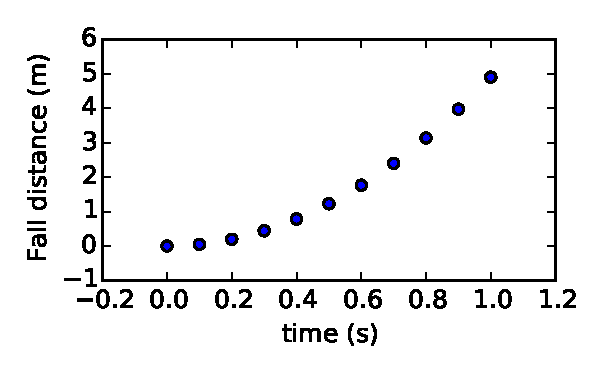
\includegraphics{Lab4_figs/yvst.pdf}
\end{center}
That is definitely not linear, but we can tweak it so that it is.  Here are the steps:
\begin{enumerate}
\item First isolate the dependent variable, or the thing you measured.  In this case, that would be our distance fallen, $y$.
\item See if it looks like a line.  Here's how you can tell. In $y=mx+b$ we have three parts that determine $y$: $m$ and $b$ are constant, $x$ is something that changes.  In our example, we change $t$ as we advance frame by frame, that's called our independent variable.
\end{enumerate}
So, let's check our equation. Do we have a constant that multiplies some function of our independent variable?  In this case, we have $\frac{1}{2}a$ as a constant, and $t^2$ is a function of our independent variable; therefore, we make our slope $m=\frac{1}{2}a$ and our x values $x=t^2$. Since we don't have anything that we are adding, $b=0$.  To add an extra check to our work, here is a plot of $y$ vs $t^2$:
\begin{center}
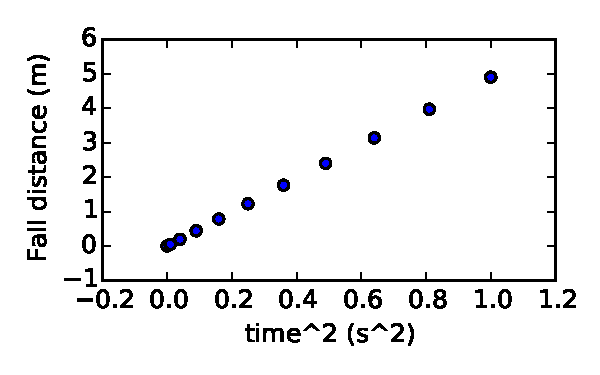
\includegraphics{Lab4_figs/yvst2.pdf}
\end{center}
which is very much linear.

As another example, suppose we wanted to find the density of copper.  To that end, we melted some copper and let it drip out a small hole, and let the drops fall as they cooled.  A drop will form an almost perfect sphere. (This is actually how they make ball bearings.)  By changing the size of the whole, you change how much mass the droplet can accumulate before it falls.  (Making mass our independent variable.)  As we vary the size of the hole, we record the mass and radius of the copper ball bearings.  Density, $\rho$, obeys the following relationship:
\[\rho = \frac{m}{V}=\frac{m}{(4/3)\pi r^3}\]

If we solve for our dependent variable, $r$, we get:
\[r^3=\frac{m}{(4/3)\pi\rho}\]
Notice that I left $r^3$, rather than solving completely for $r$.  You only need to isolate your dependent variable, not solve for it.  Our only thing that is changing on the right hand side of our equation is $m$, so our $y$ axis should be $r^3$, our $x$ axis will be $m$, and our slope will be $1/\left[\left(4/3\right)\pi\rho\right]$.

Now, we could solve completely for $r$ and get a valid result.  If we use:
\[r=\left[\frac{m}{(4/3)\pi\rho}\right]^{1/3}\]
then $r$ would be our $y$ values, $m^{1/3}$ would be our $x$ values, and $\left[\left(4/3\right)\pi\rho\right]^{-1/3}$ would be our slope.

\section{Experimental Design}

We are going to tackle the subject of experimental design today, but it helps
to have an experiment in mind. You are learning or have learned Hook's law for
springs in your PH121 class. You understand that when we attach a mass to a
spring and stretch or compress a spring we have a force
\[
F_{s}=-kx
\]
on the mass, where by $k$ we mean the spring stiffness constant, and by $x$ we
mean the displacement from the equilibrium position of the mass-spring system.
We can make such a system oscillate. This is really a PH123 problem, but let's
pretend that we are scientists in Newton's day and we don't know much about
oscillation (because most of us don't yet). We wish to find out more. We know
that if we build a mass-spring system we can get oscillation and we define the
time it takes for the mass to travel through one full oscillation (so the
mass, say, starts from the highest point and it returns to it's highest point)
as the \emph{period} of oscillation and abbreviate it with the letter $T.$
\begin{center}
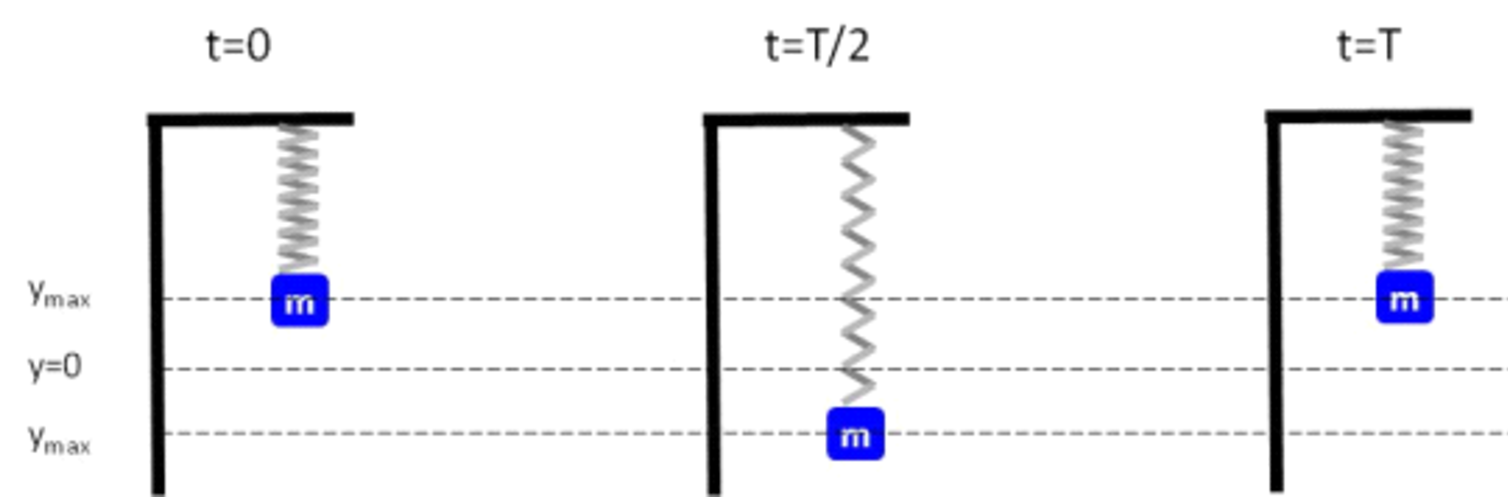
\includegraphics[width=0.5\textwidth
]
{Lab4_figs/massOnSpring.png}
\end{center}
Let's further pretend that you have read Hook's work and from this work have
reason to believe that period might be proportional to the square root of the
mass.
\[
T\propto\sqrt{m}
\]
You want to verify this report and build your own model for the period of
oscillation of a mass-spring system. You will use this model to make
predictions, and by doing so, you will see how well your model works. This is
what we want to investigate, now let's see how to design our experiment.

\section{Designing an experiment}

One of our objectives in this course is to learn how to design an experiment
so that it will be successful.

Back in grade-school, an experiment was any science related activity (the
proverbial building of a volcano model was considered an experiment). But for
a scientist, an experiment is a specific thing. It is the testing of a
hypothesis. You must test a hypothesis with care because the entire foundation
of science depends on the integrity of how we do this testing.

In this lab I will give you a hypothesis to test (the period of oscillation
for a mass-spring system depends directly on the square root of the mass). The
following steps will help your experiment be successful.

\begin{enumerate}
\item {\bf Identify the system to be examined.} In our case it is a mass-spring
system. We should identify all the \emph{inputs} to the system. For example,
we know there is a mass, $m$, and you have heard about a spring constant, $k.
$ There is also the force due to gravity and tension on a spring. These are
inputs. You should describe your system in your lab notebook and list the
inputs. These inputs are the things you can possibly change in the design of
your experiment.

\item {\bf Identify the model to be tested.} The word \textquotedblleft
model\textquotedblright\ means our mental picture of how something works. As
physicists, we would prefer to express a model in a mathematical equation. For
example, we have a model of how force depends on acceleration. The bigger the
acceleration, the more the force. But our model also includes mass. The larger
the mass, the larger the force needed to create the same acceleration. This
mental model can be expressed in an equation
\[
F=ma
\]
It is valuable to use both the word description of the model as well as our
mathematical representation. In our case today, our mental model is that
period of oscillation for a mass-spring system depends directly on the square
root of the mass. Think about what this means. If I increase the mass, the
period should get longer. But if I\ double the mass, the period won't double.
This is a mental model that allows us to do predictions of behavior. In
physics it is almost required to reduce this model to an algebraic equation
that can be used to calculate a prediction and an uncertainty on that
prediction. For today's experiment that equation is
\[
T=C\sqrt{m}
\]
where $C$ is a factor that does not depend on mass, but for your experiment
that your group designs later in this course you will have to come up with
your own mathematical expression of your model. Record your model and the
model equation in your lab notebook.

\item {\bf Plan how you will know if you are successful in your experiment.} You are
testing a hypothesis, and you are much more likely to succeed in your test if
you plan what that success would look like. One way to do this is to plan how
you will communicate your results. It is a great idea to think of what graph
you will make at the end of the experiment to communicate whether your model
works (or not). In today's experiment, a graph of $T$ vs. $m$ or even $T$
vs.$\sqrt{m}$ might be useful along with a curve fit. Notice I\ am suggesting
you plan this before you perform the experiment. I am not suggesting you
decide on what the results will be, only how you will report them. This
focuses your attention on deciding what measurement you will make. In our case
today it is hard to plot $T$ vs. $m$ if you don't measure $T$ and $m,$
planning the graph in advance helps you plan the experiment. Mock up your
graph or figure in your lab notebook. Give axis titles and even units (but of
course no data yet).

\item {\bf Plan your analysis.}  Symbolically layout and solve any needed equations.  That way you will know exactly what measurements you need to make, and will not have to try to recreate the experiment when you are analyzing your results.

If possible, rectify (linearize) your equation. It would be good to be able to use a curve fit to
analyze our data. The strongest and most reliable curve fits are straight line
fits where the fit equation is something like
\[
y=mx+b
\]
So if at all possible, we would like to reduce our equation to the equation of
a straight line. In today's lab we can do this. We call this \emph{linearizing
the equation}. If we can't find a way to linearize the equation, we at least
need to render our equation into a form that we can use to predict the outcome
of our experiment. Record your new equation in your lab notebook.

\item {\bf Choose ranges of the variables.} For today's experiment we might have
several, but $m$ and $k$ are principal variables. It should be clear when you
see the spring that putting a thousand kilograms of mass on the spring would
be a bad idea. but how much mass is right? What will give you good results in
testing your theory? Hooks law is not valid for all $m$ and $k$ (if you doubt
this, think of your Christmas slinky after your brother got to it; it never
looked the same again!). What values of $m$ are best for performing the
experiment? An error analysis based on your equation is invaluable in making
this decision. Changes in mass that produce a change in $T$ that is smaller
than the uncertainty in $T$ will not be noticeable. So taking measurements for
such small mass changes would be a waste of time and effort. We would like to
avoid this. Changes that are likely to break the equipment are also not
desirable. And of course you want to plan this before you do the experiment
and find that you did not get good data, and therefore must repeat all your
work! Record your variable ranges in your lab notebook. As you perform the
experiment note any deviations from this plan.

\item {\bf Plan the experimental procedure.} As a group talk your way through the
experiment. You might find yourselves saying something like ``
Then you take the stopwatch and measure the period." and
you realize that you did not get a stop watch. For your experiment that you
design, you need to find out in advance if we have the equipment you need. So
get in the habit of working through the procedure in advance to see if you
have forgotten anything. Record your planned procedure in your lab notebook.
As you perform the experiment, note any deviations from the plan and the
reason for the deviation. Deviations are fine, just make sure you record them.

\item {\bf Perform the experiment and report on it in your lab notebook.} This
involves all the things we have been including in our lab notebooks to date:


\begin{itemize}
\item Describing the goal for the work. (This is probably already done in your plan)

\item Give predictive equations and uncertainties for the predictions based on
the physical law. (This is probably already done in your plan)

\item Give your procedure you actually followed, recording what you really did
as you do it. This will probably not be just a restatement of the plan because
things will change as you go. Record the equipment used and settings, values,
etc. for that equipment. Did you learn how to use any new equipment? What did
you learn that you want to recall later (say, when taking the final, or when
you are a professional and need to use a similar piece of equipment five years
from now).

\item Record the data you used. If you have a large set of values, you can
place them in a file, and then record the file name and location in your lab
notebook. Make sure this is a file location that does not change (emailing the
data to yourself is still not a good plan).

\item Give a record of the analysis you performed. You planned this above, now
record what you actually did

\item Give a brief statement of your results and their associated uncertainties.

\item Draw conclusions: Do your results support the theory? Why or why not?
What else did you learn along the way that you want to record. (This is where
we may compare the percent error to our relative uncertainty).
\end{itemize}
\end{enumerate}


\end{document}


\part{Lab Assignments}
%Start Counting Back at 1
\setcounter{chapter}{0}
\renewcommand{\chaptername}{Lab}

\documentclass[twoside,11pt,ShortChapTitles]{BYUTextbook}

\usepackage{soul}
\renewcommand{\vec}[1]{\ensuremath{\mathbf{#1}}}
\usepackage{siunitx}
\sisetup{round-mode = figures,
  round-precision = 3, scientific-notation=true}
  \usepackage{marginfix}
  
\usepackage{mathtools}
%\usepackage{amsfonts}
%\usepackage{amsmath}
%\usepackage{graphicx}
%\usepackage{epstopdf}
%\usepackage{amssymb}
%\usepackage{hyperref}
%\usepackage{textcomp}
%\usepackage{listings}
%\usepackage{units}
%\usepackage{color}

%\definecolor{dkgreen}{rgb}{0,0.6,0}
%\definecolor{gray}{rgb}{0.5,0.5,0.5}
%\definecolor{mauve}{rgb}{0.58,0,0.82}

%\lstset{frame=tb,
%  language=Python,
%  aboveskip=3mm,
%  belowskip=3mm,
%  showstringspaces=false,
%  columns=flexible,
%  basicstyle={\small\ttfamily},
%  numbers=none,
%  numberstyle=\tiny\color{gray},
%  keywordstyle=\color{blue},
%  commentstyle=\color{dkgreen},
%  stringstyle=\color{mauve},
%  breaklines=true,
%  breakatwhitespace=true,
%  tabsize=3, upquote=true}
\renewcommand{\chaptername}{Lab}
\lstMakeShortInline[columns=fixed]|
\setcounter{chapter}{0}

\begin{document}

\chapter{Measurement and Uncertainty I\label{Measurement and Uncertainty 1}}

\setcounter{page}{1}

\section{Lab Notebooks}

Hopefully you noticed that a lab notebook is required for this class. The lab
notebook is designed to be a record of what you did. If you had to repeat
today's experiment five years from now, could you do it based on what you
write today?

At most professional labs and major engineering companies your lab notebook is
considered the property of the company or organization and will stand as a legal document. It is the proof that
you did the experiment that you say you did, and that you got the results you
say you got. It has to be readable and understandable to someone who did not
participate in the lab with you. This is a pretty tall order. 

{\em You should write  in your lab notebook as you go}, not leave it until the end of the day\sidenote{A lab notebook is not a lab report.  You just nned to take well organized notes on what you did and what you found.}.  It will be much easier, and will take you less time as you go.   To help you plan your entries, here are the criteria I will use to grade your lab book:

\begin{itemize}
\item Describing the goal for the work

\begin{itemize}
\item Usually this takes the form of a physical law we will test.
\end{itemize}

\item Give predictive equations and uncertainties for the predictions based on
the physical law.

\begin{itemize}
\item This usually involves forming a mathematical model. You should record
any assumptions that went into the model (e.g. no air resistance, point
sources, massless ropes, etc.).

\begin{itemize}
\item In lab today we will find the volume of the room. Your mathematical
model will likely be $V=\ell\times w\times h.$ The mathematical model is not
necessarily something complicated, but the reader needs to know how you are
doing your calculations.
\end{itemize}
\end{itemize}

\item Give your procedure

\begin{itemize}
\item Recording what you really did (not the lab instructions), tell what
changes you make in your procedure as you make them.

\item Record as you do the work.

\item Record the equipment used and settings, values, etc. for that equipment
(see next item).

\item Did you learn how to use any new equipment? What did you learn that you
want to recall later (say, when taking the final, or when you are a
professional and need to use a similar piece of equipment five years from now).
\end{itemize}

\item Record the data you used. The data are all the measurements you took
plus your best estimate of the uncertainties in the measurements. Record any
values you got from tables or published sources (or from your professor) and
state where you got these values. You don't always want to write down all the
data you use. If you have a large set of values, you can place them in a file,
and then record the file name and location in your lab notebook. Make sure
this is a file location that does not change (emailing the data to yourself is
not a good plan).

\item Give a record of the analysis you performed. You should have given some
idea of how you got your predictive equation. Now, what did you do to get the
data through the equation? Were there any extra calculations? Did you obtain a
set of  ``truth data" (data from tables or
published sources, or from an alternate experiment) for your experiment? If
so, did you do any calculations, have any uncertainty, etc. associated with
the truth values?

\item Give a brief statement of your results and their associated uncertainties.

\item Draw conclusions

\begin{itemize}
\item Do your results support the theory? Why or why not? What else did you
learn along the way that you want to record.

\item This is where we may compare the percent error to our relative uncertainty.
\end{itemize}
\end{itemize}



\section{Assignment: Practice with Measurement and Uncertainty calculations.}

\subsection{Part 1 Percent Error: Mass of a Cylinder--the hard way}

\begin{itemize}
\item Given the density of a metal cylinder, use this density to determine the
mass the cylinder.

\begin{itemize}
\item You cannot directly measure the mass of the cylinder, You will be
provided a mass of the cylinder by your instructor to compare with your
calculated value.

\item Report your method for obtaining the mass of the cylinder in your lab
notebook (not just your result, but tell yourself in your notebook \emph{how
you got your result}).

\item Report the following results: 1) Density of the cylinder, 2) Predicted
Mass of the cylinder, 3) Actual Mass of the cylinder. Comment on the accuracy
and precision of your measurement.

\item Resources: You may use any equipment or other resources found in the lab
or on the internet
\end{itemize}
\end{itemize}

\subsection{Part 2 Combining Uncertainty: Volume of the room}

\begin{itemize}
\item Determine the volume of this room, including uncertainties. Describe
your method fully in your lab notebook, including which measuring instruments
you used and why, and the uncertainty in each of your measurements.

\item The relative uncertainty in the volume is
\[
\frac{\delta V}{V}=\frac{\delta L}{L}+\frac{\delta H}{H}+\frac{\delta W}{W}
\]
from Taylor's equation 2.28 or from our algebraic method multiplication rule.

\item Compare your answers with those from your neighboring research
institutions at the other tables. Are your answers the same to within the
values of your uncertainty? If not, explain why they aren't.
\end{itemize}

\subsection{Part 3: Tie to Experimentation}

\begin{itemize}
\item We will learn in this class that you should understand the uncertainties
in our measuring devices \emph{before} you start performing an experiment.
From what you have experienced so far today, why do you think this is so?
\end{itemize}

\subsection{Part 4 Combining Uncertainty: Determine the Volume of a Stack of
Paper}

\begin{itemize}
\item Determine the volume of $20$ pieces of paper (you can use more, but if
you do, replace the number $20$ with your actual number in the equation below).

\item Determine the uncertainty in your measurement.

\item Use your measurement to find the volume of one sheet of paper by
dividing. Also determine the uncertainty in your calculation. This should be
something like
\[
\delta V_{1}=\frac{\delta V_{20}}{20}
\]
explain what this means in your lab notebook.

\item Now measure the volume of one piece of paper directly using instruments
(I might recommend a micrometer--ask if you have not used one before).

\item How do your measurements compare?

\item Which one is more accurate? Which is more precise? Why?
\end{itemize}



\end{document}

% END OF DOCUMENT =======================================================


%SECTION ON LAB NOTEBOOKS =================================================



%END SECTION ON LAB NOTEBOOKS ==============================================



%EXCISED MATERIAL==================================================

We can see that if you have $z=x+y$ then you just add the uncertainties
$\delta z=\delta x+\delta y.$ Of course $z$, $x,$ and $y$ stand for any
variable. But how do we know this is true? Here are the details of how the
algebraic method works

\subsubsection{Multiplication}

To multiply two measurements, say\[
m_{measured}=m_{N}\pm\delta m
\]\[
v_{measured}=v_{N}\pm\delta v
\]


We could write these as\[
m_{measured}=m_{N}\left(  1\pm\frac{\delta m}{\left\vert m_{N}\right\vert
}\right)
\]\[
v_{measured}=v_{N}\left(  1\pm\frac{\delta v}{\left\vert v_{N}\right\vert
}\right)
\]


This gives us the measurement in terms of the fractional uncertainties. If we
wish to compute
\[
p=mv
\]
we use
\[
p_{N}=m_{N}v_{N}
\]
but what is the uncertainty in $p?$

The largest value of $p$ is given by\[
p_{\text{large}}=m_{\mathbf{N}}v_{\mathbf{N}}\left(  1+\frac{\delta
m}{\left\vert m_{N}\right\vert }\right)  \left(  1+\frac{\delta v}{\left\vert
v_{\mathbf{N}}\right\vert }\right)
\]
which can be written as\[
p_{\text{large}}=m_{\mathbf{N}}v_{\mathbf{N}}\left(  1+\frac{\delta
m}{\left\vert m_{\mathbf{N}}\right\vert }+\frac{\delta v}{\left\vert
v_{\mathbf{N}}\right\vert }+\frac{\delta v}{\left\vert v_{\mathbf{N}}\right\vert }\frac{\delta m}{\left\vert m_{\mathbf{N}}\right\vert }\right)
\]
We reason that fractional uncertainties should be small, so products of
fractional uncertainties should be very small. We will ignore the very small
term\[
\frac{\delta m}{\left\vert v_{\mathbf{N}}\right\vert }\frac{\delta
m}{\left\vert m_{\mathbf{N}}\right\vert }
\]
so we have\[
p_{\text{large}}=m_{\mathbf{N}}v_{\mathbf{N}}\left(  1+\frac{\delta
m}{\left\vert m_{\mathbf{N}}\right\vert }+\frac{\delta v}{\left\vert
v_{\mathbf{N}}\right\vert }\right)
\]
The smallest value of $p$ is likewise\[
p_{\text{small}}=m_{\mathbf{N}}v_{\mathbf{N}}\left(  1-\frac{\delta
m}{\left\vert m_{\mathbf{N}}\right\vert }-\frac{\delta v}{\left\vert
v_{\mathbf{N}}\right\vert }\right)
\]
In each case we have $m_{\mathbf{N}}v_{\mathbf{N}}$ and then either plus or
minus the term $\frac{\delta m}{\left\vert m_{\mathbf{N}}\right\vert }+\frac{\delta v}{\left\vert v_{\mathbf{N}}\right\vert }$so we have, for our
calculated value of $p$\[
p_{\text{calculated}}=m_{\mathbf{N}}v_{\mathbf{N}}\left(  1\pm\left(
\frac{\delta m}{\left\vert m_{\mathbf{N}}\right\vert }+\frac{\delta
v}{\left\vert v_{\mathbf{N}}\right\vert }\right)  \right)
\]
which we must be able to write as a nominal value and an uncertainty in $p$\[
p_{\text{calculated}}=p_{\mathbf{N}}\left(  1\pm\frac{\delta p}{\left\vert
p_{\mathbf{N}}\right\vert }\right)
\]
Comparing the previous two equations we can see that we must have\[
\frac{\delta p}{\left\vert p_{\mathbf{N}}\right\vert }=\left(  \frac{\delta
m}{m_{\mathbf{N}}}+\frac{\delta v}{v_{\mathbf{N}}}\right)
\]


Then when we multiple measured quantities, we add fractional uncertainties.
This is our algebraic rule for multiplication.

Don't forget, that we need to report $\delta p,$ so to find $\delta p$ we
take\[
\delta p=\frac{\delta p}{\left\vert p_{\mathbf{N}}\right\vert }p_{\mathbf{N}}
\]


\subsubsection{Division}

Let's start again with two measured values $x$ and $y$ with the form\[
x=x_{\mathbf{N}}\left(  1\pm\frac{\delta x}{\left\vert x_{\mathbf{N}}\right\vert }\right)
\]\[
y=y_{\mathbf{N}}\left(  1\pm\frac{\delta y}{\left\vert y_{\mathbf{N}}\right\vert }\right)
\]
We can find the quotient
\[
q=q_{\mathbf{N}}\pm\delta q
\]
as we did for multiplication\[
q=\frac{x_{\mathbf{N}}\left(  1\pm\frac{\delta x}{\left\vert x_{\mathbf{N}}\right\vert }\right)  }{y_{\mathbf{N}}\left(  1\pm\frac{\delta y}{\left\vert
y_{\mathbf{N}}\right\vert }\right)  }
\]
Again find the maximum quotient\[
q_{\text{large}}=\frac{x_{\mathbf{N}}\left(  1+\frac{\delta x}{\left\vert
x_{\mathbf{N}}\right\vert }\right)  }{y_{\mathbf{N}}\left(  1-\frac{\delta
y}{\left\vert y_{\mathbf{N}}\right\vert }\right)  }
\]
and we will play a mathematical trick, we will multiple both top and bottom by
$\left(  1+\frac{\delta y}{\left\vert y_{\mathbf{N}}\right\vert }\right)
,$ since
\[
\frac{\left(  1+\frac{\delta y}{\left\vert y_{\mathbf{N}}\right\vert }\right)
}{\left(  1+\frac{\delta y}{\left\vert y_{\mathbf{N}}\right\vert }\right)
}=1
\]
this will not change our value for $q_{\text{large}}$\[
q_{\text{large}}=\frac{x_{\mathbf{N}}\left(  1+\frac{\delta x}{\left\vert
x_{\mathbf{N}}\right\vert }\right)  }{y_{\mathbf{N}}\left(  1-\frac{\delta
y}{\left\vert y_{\mathbf{N}}\right\vert }\right)  }\frac{\left(
1+\frac{\delta y}{\left\vert y_{\mathbf{N}}\right\vert }\right)  }{\left(
1+\frac{\delta y}{\left\vert y_{\mathbf{N}}\right\vert }\right)  }
\]
The denominator is\[
y_{\mathbf{N}}\left(  1-\frac{\delta y}{\left\vert y_{\mathbf{N}}\right\vert
}\right)  \left(  1+\frac{\delta y}{\left\vert y_{\mathbf{N}}\right\vert
}\right)
\]
We can perform the multiplication to get\begin{align*}
& y_{\mathbf{N}}\left(  1-\frac{\delta y}{\left\vert y_{\mathbf{N}}\right\vert
}+\frac{\delta y}{\left\vert y_{\mathbf{N}}\right\vert }-\frac{\delta
y}{\left\vert y_{\mathbf{N}}\right\vert }\frac{\delta y}{\left\vert
y_{\mathbf{N}}\right\vert }\right) \\
& =y_{\mathbf{N}}\left(  1-\frac{\delta y}{\left\vert y_{\mathbf{N}}\right\vert }\frac{\delta y}{\left\vert y_{\mathbf{N}}\right\vert }\right)
\end{align*}
and we can perform the multiplication in the numerator
\[
x_{\mathbf{N}}\left(  1+\frac{\delta x}{\left\vert x_{\mathbf{N}}\right\vert
}+\frac{\delta y}{\left\vert y_{\mathbf{N}}\right\vert }+\frac{\delta
x}{\left\vert x_{\mathbf{N}}\right\vert }\frac{\delta y}{\left\vert
y_{\mathbf{N}}\right\vert }\right)
\]
so\[
q_{\text{large}}=\frac{x_{\mathbf{N}}\left(  1+\frac{\delta x}{\left\vert
x_{\mathbf{N}}\right\vert }+\frac{\delta y}{\left\vert y_{\mathbf{N}}\right\vert }+\frac{\delta x}{\left\vert x_{\mathbf{N}}\right\vert }\frac{\delta y}{\left\vert y_{\mathbf{N}}\right\vert }\right)  }{y_{\mathbf{N}}\left(  1-\frac{\delta y}{\left\vert y_{\mathbf{N}}\right\vert
}\frac{\delta y}{\left\vert y_{\mathbf{N}}\right\vert }\right)  }
\]
The term\[
\frac{\delta y}{\left\vert y_{\mathbf{N}}\right\vert }\frac{\delta
y}{\left\vert y_{\mathbf{N}}\right\vert }
\]
is very small compared to $1$ (if $\delta y/\left\vert y_{\mathbf{N}}\right\vert $ is a small number, as we assume, then $\delta y^{2}/\left\vert
y_{\mathbf{N}}\right\vert ^{2}$ will be very tiny) so we will drop it from
our calculations (we are calculating uncertainty, the fifth decimal place in
the uncertainty is very uncertain!). We can do this as well with the term\[
\frac{\delta x}{\left\vert x_{\mathbf{N}}\right\vert }\frac{\delta
y}{\left\vert y_{\mathbf{N}}\right\vert }
\]
like we did with the multiplication case. Then\begin{align*}
q_{\text{large}}  & =\frac{x_{\mathbf{N}}\left(  1+\frac{\delta x}{\left\vert
x_{\mathbf{N}}\right\vert }+\frac{\delta y}{\left\vert y_{\mathbf{N}}\right\vert }\right)  }{y_{\mathbf{N}}\left(  1\right)  }\\
& =\frac{x_{\mathbf{N}}}{y_{\mathbf{N}}}\left(  1+\frac{\delta x}{\left\vert
x_{\mathbf{N}}\right\vert }+\frac{\delta y}{\left\vert y_{\mathbf{N}}\right\vert }\right)
\end{align*}
We could go through this again for $q_{\text{small}}$ and we would find
\begin{align*}
q_{\text{small}}  & =\frac{x_{\mathbf{N}}\left(  1-\left(  \frac{\delta
x}{\left\vert x_{\mathbf{N}}\right\vert }+\frac{\delta y}{\left\vert
y_{\mathbf{N}}\right\vert }\right)  \right)  }{y_{\mathbf{N}}\left(  1\right)
}\\
& =\frac{x_{\mathbf{N}}}{y_{\mathbf{N}}}\left(  1-\left(  \frac{\delta
x}{\left\vert x_{\mathbf{N}}\right\vert }+\frac{\delta y}{\left\vert
y_{\mathbf{N}}\right\vert }\right)  \right)
\end{align*}


We can then write\begin{align*}
q_{\text{calculated}}  & =\frac{x_{\mathbf{N}}}{y_{\mathbf{N}}}\left(
1\pm\left(  \frac{\delta x}{\left\vert x_{\mathbf{N}}\right\vert }+\frac{\delta y}{\left\vert y_{\mathbf{N}}\right\vert }\right)  \right) \\
& =q_{\mathbf{N}}\left(  1\pm\frac{\delta q}{\left\vert q\right\vert }\right)
\end{align*}
where
\[
q_{\mathbf{N}}=\frac{x_{\mathbf{N}}}{y_{\mathbf{N}}}
\]
and\[
\frac{\delta q}{\left\vert q\right\vert }=\frac{\delta x}{\left\vert
x_{\mathbf{N}}\right\vert }+\frac{\delta y}{\left\vert y_{\mathbf{N}}\right\vert }
\]
just like the formula for multiplication! The rule is when we divide measured
quantities, we add fractional uncertainties

\subsubsection{Addition}

Let's take two measurements\[
x_{measured}=x_{\mathbf{N}}\pm\delta x
\]\[
y_{measured}=y_{\mathbf{N}}\pm\delta y
\]
and add them to get the largest value of the sum, $z$\begin{align*}
z_{\text{large}}  & =x_{measured}+y_{measured}\\
& =x_{\mathbf{N}}+y_{\mathbf{N}}+\delta x+\delta y
\end{align*}
We can also find the smallest value for $z$\begin{align*}
z_{\text{small}}  & =x_{measured}+y_{measured}\\
& =x_{\mathbf{N}}+y_{\mathbf{N}}-\left(  \delta x+\delta y\right)
\end{align*}
so if we write this as $z_{\mathbf{N}}\pm\delta z$ we have\[
z_{\mathbf{N}}\pm\delta z=x_{\mathbf{N}}+y_{\mathbf{N}}\pm\left(  \delta
x+\delta y\right)
\]
and we can identify
\begin{align*}
z_{\mathbf{N}}  & =x_{\mathbf{N}}+y_{\mathbf{N}}\\
\delta z  & =\left(  \delta x+\delta y\right)
\end{align*}


The rule is that when we add measurements we add their uncertainties.

\subsubsection{Subtraction}

Let's take two measurements\[
x_{measured}=x_{\mathbf{N}}\pm\delta x
\]\[
y_{measured}=y_{\mathbf{N}}\pm\delta y
\]
and add them to get the largest value of the sum, $z$\begin{align*}
z_{\text{large}}  & =x_{measured}-y_{measured}\\
& =\left(  x_{\mathbf{N}}+\delta x\right)  -\left(  y_{\mathbf{N}}-\delta
y\right)
\end{align*}
We can also find the smallest value for $z$\begin{align*}
z_{\text{small}}  & =x_{measured}-y_{measured}\\
& =\left(  x_{\mathbf{N}}-\delta x\right)  -\left(  y_{\mathbf{N}}+\delta
y\right)
\end{align*}
so if we write this as $z_{\mathbf{N}}\pm\delta z$ we have\[
z_{\mathbf{N}}\pm\delta z=x_{\mathbf{N}}-y_{\mathbf{N}}\pm\left(  \delta
x+\delta y\right)
\]
and we can identify
\begin{align*}
z_{\mathbf{N}}  & =x_{\mathbf{N}}-y_{\mathbf{N}}\\
\delta z  & =\left(  \delta x+\delta y\right)
\end{align*}


The rule is that when we subtract measurements, we add their uncertainties
just as we found for addition.

\subsubsection{Measured quantity times an exact number}

Suppose we want the circumference of a circle. We measure the radius to be\[
r_{measured}=r_{\mathbf{N}}\pm\delta r
\]
and we calculate
\[
C_{calculated}=2\pi r_{measured}
\]
how do we determine the uncertainty?

There is not uncertainty in the $2$ nor in the $\pi.$ So we multiply\begin{align*}
C_{calc}  & =2\pi\left(  r_{\mathbf{N}}\pm\delta r\right) \\
& =2\pi r_{\mathbf{N}}\pm2\pi\delta r
\end{align*}
which gives
\[
C_{\mathbf{N}}\pm\delta C=2\pi r_{\mathbf{N}}\pm2\pi\delta r
\]
and we identify
\[
C_{\mathbf{N}}=2\pi r_{\mathbf{N}}
\]
and
\[
\delta C=2\pi\left\vert \delta r\right\vert
\]


In general, if we have
\[
q=Bx
\]
where $B$ is a constant, then we should expect\[
\delta q=\left\vert B\right\vert \delta x
\]


\paragraph{Powers}

For a power, we really are just multiplying\[
y=x^{2}=x\times x
\]
so, taking the fractional uncertainty rule for multiplication,\begin{align*}
\frac{\delta y}{\left\vert y\right\vert }  & =\frac{\delta x}{\left\vert
x\right\vert }+\frac{\delta x}{\left\vert x\right\vert }\\
& =2\frac{\delta x}{\left\vert x\right\vert }\end{align*}


In general, if
\[
y=x^{n}
\]
then
\[
\frac{\delta y}{\left\vert y\right\vert }=n\frac{\delta x}{\left\vert
x\right\vert }
\]


\documentclass{book}%
\usepackage{amsfonts}
\usepackage{amsmath}%
\usepackage{graphicx}
\usepackage{epstopdf}
\usepackage{amssymb}%
\usepackage{hyperref}
\usepackage{textcomp}
\usepackage{listings}
\usepackage{units}
\usepackage{color}

\definecolor{dkgreen}{rgb}{0,0.6,0}
\definecolor{gray}{rgb}{0.5,0.5,0.5}
\definecolor{mauve}{rgb}{0.58,0,0.82}

\lstset{frame=tb,
  language=Python,
  aboveskip=3mm,
  belowskip=3mm,
  showstringspaces=false,
  columns=flexible,
  basicstyle={\small\ttfamily},
  numbers=none,
  numberstyle=\tiny\color{gray},
  keywordstyle=\color{blue},
  commentstyle=\color{dkgreen},
  stringstyle=\color{mauve},
  breaklines=true,
  breakatwhitespace=true,
  tabsize=3, upquote=true}

\lstMakeShortInline[columns=fixed]|




\setcounter{chapter}{1}

\begin{document}

\chapter[Statistical Representation of Data]{Communicating Results I: Statistical Representation of Data}

So far we have talked about repeating experiments, but we have been too
pressed for time to actually do that. We should take the time to see how to
report data from multiple results. Let's also tie the idea of multiple
results to our ideas of uncertainty.

To do this, I would like to go back to our dart board. Suppose I throw the
darts, trying for a bull's eye, and I get the following pattern:

\begin{center}
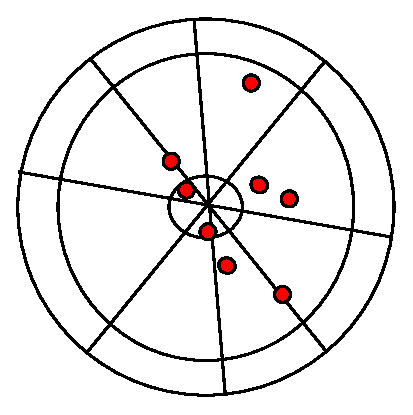
\includegraphics[scale=0.5]{Lab2_figs/bullseye_few.eps}
\end{center}

We now know that this is fairly accurate, but not very precise. We say that
there is a large uncertainty, but that we are aimed about the right
direction. We could get a better estimate of how accurate we are by
repeating the experiment many times:

\begin{center}
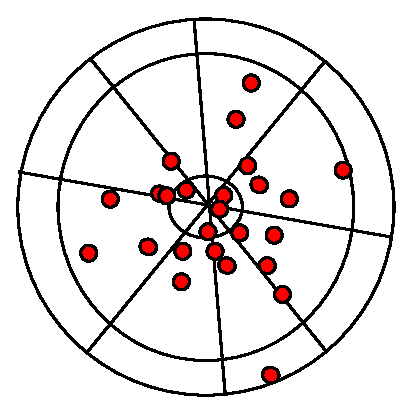
\includegraphics[scale=0.5]{Lab2_figs/bullseye_many.eps}
\end{center}

and finding an average location of the darts:

\begin{center}
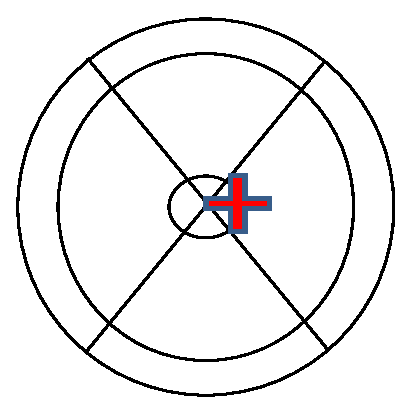
\includegraphics[scale=0.5]{Lab2_figs/bullseye_avg.eps}
\end{center}

This average seems to be just a little right of center. Now we know that we should point the darts a little
to the left. Many experiments are like this. We can repeat the experiment
many times. The uncertainty might be larger than we want, but if we average
over many trials of the experiment, we can find an average value that
represents the actual value of the quantity we are trying to find.

\section{Mean value as our best estimate value}

The mathematical process we use to find the mean is simple and you are
probably quite familiar with it. We simply add up all the values, and divide
the sum by the number of values.%
\begin{eqnarray*}
\bar{x} &=&\frac{x_{1}+x_{2}+x_{3}+\cdots x_{N}}{N} \\
&=&\frac{1}{N}\sum_{i=1}^{N}x_{i}
\end{eqnarray*}%
The last equation uses sigma notation. It is read as \textquotedblleft one
over $N$ times the sum of $x_{i}$ for $i=1$ to $N.$ It is a short-hand
notation for the line above. We will use this notation because it makes
writing our equations much easier. But that means it is very important that
we understand what it means. So let's imagine that we have many values for
the $x$-position for our darts.%
\[
\begin{array}{c}
x_{1}=1.00\pm 0.01\unit{cm} \\ 
x_{2}=0.50\pm 0.01\unit{cm} \\ 
x_{3}=-0.75\pm 0.01\unit{cm} \\ 
x_{4}=-2.25\pm 0.01\unit{cm} \\ 
x_{5}=3.00\pm 0.01\unit{cm} \\ 
x_{6}=-0.80\pm 0.01\unit{cm} \\ 
x_{7}=2.10\pm 0.01\unit{cm} \\ 
x_{8}=1.2\pm 0.01\unit{cm}%
\end{array}%
\]%
We have labeled each $x$ with a number. That is what the $x_{i}$ means. The
\textquotedblleft $i$\textquotedblright\ is an index. It stands for any
number from $1$ to $N.$ Our sigma notation says we add up all these
positions, and divide by $N=8$ since there are eight positions%
\begin{eqnarray*}
\bar{x} &=&\frac{\left( 1.00+0.50-0.75-2.25+3.00-0.80+2.10+1.2\right) \unit{%
cm}}{8} \\
&=&0.5\unit{cm}
\end{eqnarray*}%
which is a little bit to the right of our zero point.

\section{Standard deviation as an estimate of our uncertainty}

But what is our uncertainty? Each of our position measurements were good to $%
\pm 0.01\unit{cm}.$ But this can't be what governs our uncertainty. We can
see our points are spread out much more than $\pm 0.01\unit{cm}.$ Something
in the experiment (the bad dart thrower) is increasing the uncertainty. We
could use our algebraic method to find the uncertainty, but that would be
tedious and may not include the effects of the dart thrower. It would be
great to have a way to use the spread of the points, itself, to obtain a
numerical estimate of the uncertainty. The spread must include the effects
of the dart thrower.

From your study of statistics, you can guess what we will use to represent
uncertainty, but let's reason it out here. We could take how far each point
is from where we aimed as an indication of how imprecise our throw was. That
would be 
\[
\Delta x_{i}=\bar{x}-x_{i} 
\]%
for each throw. In this equation we are using the Greek $\Delta $ to show a
difference, and a bar over the $x$ to mean \textquotedblleft the average
value of the $x$-position.\textquotedblright\ Then $\Delta x_{i}$ is how far
off the $i^{th}$ trow from the mean. Sometimes we are off to the right, and
sometimes to the left. If we add up all the $\Delta x_{i}$ values and
average them, they will average to nearly zero most of the time. We can see
that zero is not a good estimate of our uncertainty! So the average
deviation won't work as a measure of uncertainty.

But we can play a trick. The quantity 
\[
\Delta x_{i}^{2}=\left( \bar{x}-x_{i}\right) ^{2} 
\]%
is always positive. If we averaged $\Delta x_{i}^{2},$ 
\[
\overline{\Delta x_{i}^{2}}=\frac{1}{N}\sum_{i=1}^{N}\Delta x_{i}^{2}=\frac{1%
}{N}\sum_{i=1}^{N}\left( \bar{x}-x_{i}\right) ^{2} 
\]%
nothing would cancel out. And we have solved our calcelation problem. But we
have created another problem by doing this, $\overline{\Delta x_{i}^{2}}$ is
like the square of our how far we are off. So let's take a square root%
\[
\sqrt{\overline{\Delta x_{i}^{2}}}=\sqrt{\frac{1}{N}\sum_{i=1}^{N}\Delta
x_{i}^{2}}=\sqrt{\frac{1}{N}\sum_{i=1}^{N}\left( \bar{x}-x_{i}\right) ^{2}} 
\]%
The quantity $\sqrt{\overline{\Delta x_{i}^{2}}},$ represents about how far
off we are on average, it does not tend to zero, and has the same units as $%
x_{i}$ so it can be an estimate of our uncertainty. It is about how far most
of the points are off from the mean. But $\sqrt{\overline{\Delta x_{i}^{2}}}$
is a little hard to write, so we usually give this quantity the symbol $%
\sigma $, which is a Greek letter $s$ and is pronounced \textquotedblleft
sigma.\textquotedblright\ We also give $\sigma $ a name. We call it the 
\emph{standard deviation} because it is about how much the average point
\textquotedblleft deviates\textquotedblright\ from the mean position. So for
our $x$-position we can write 
\[
\sigma _{x}=\sqrt{\sum_{i=1}^{N}\frac{\left( x_{i}-\bar{x}\right) ^{2}}{N}} 
\]%
But what does this math symbology mean? To find $\sigma _{x},$ we must first
find the average positions to find $\bar{x},$ then we take each $x$-position 
$\left( x_{i}\right) $ and we subtract the mean from it $\left( x_{i}-\bar{x}%
\right) .$ We square the result. We do this for each of our $x$-positions.
Then we have $\left( x_{1}-\bar{x}\right) ^{2},$ $\left( x_{2}-\bar{x}%
\right) ^{2},$ $\left( x_{3}-\bar{x}\right) ^{2},\cdots \left( x_{N}-\bar{x}%
\right) ^{2}.$ We add these up, and divide by $N$ to find the average $%
\sum_{i=1}^{N}\frac{\left( x_{i}-\bar{x}\right) ^{2}}{N}.$ Then we take the
square root.

In lab today, I\ will ask you to do this by hand once. That should be enough
to convince you that you never want to do it by hand again! Normally we will
use a computer to do this. I suggest you use one of our spreadsheet
programs, or python to do these calculations, and not your calculator.

\section{Histograms}

Suppose I\ plot the results of many, many dart throws. The way I want to
plot this is something you have seen from grading for many years. I want the
horizontal axis to show the $x$-position of the dart throws. I want the $y$%
-axis to show the number of darts that landed at a particular $x$-position.
This type of graph is called a histogram. You often see grades given like
this

\begin{center}
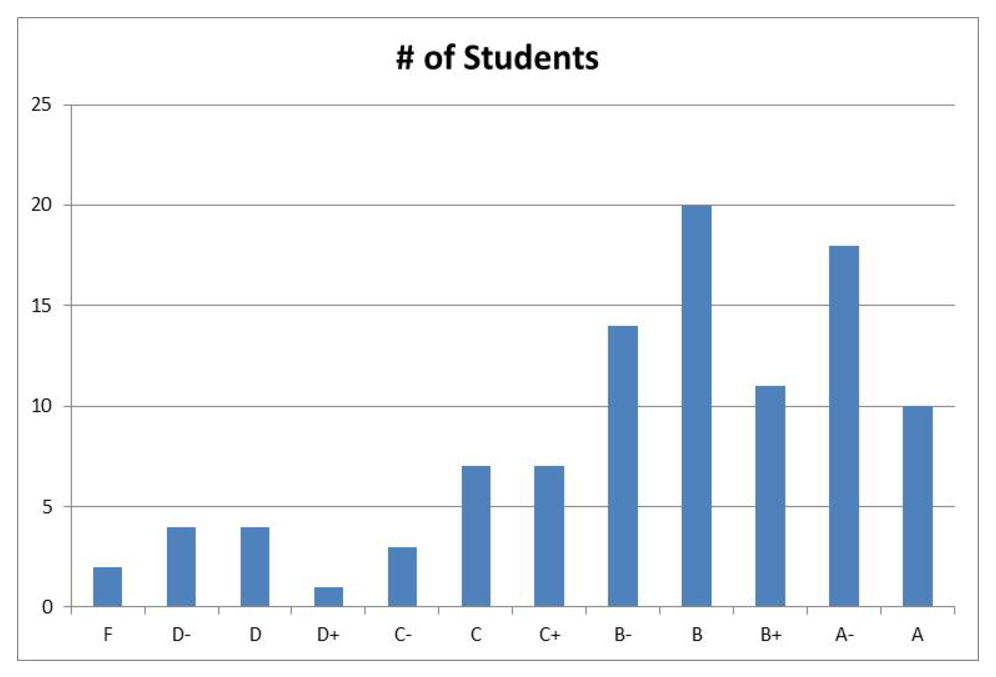
\includegraphics[scale=0.5]{Lab2_figs/hist_few.eps}
\end{center}

where we understand that the bars
indicate how many students got an $A$ (two in this case) and how many got an 
$A-$ (five in this case) etc.

If there are many students we can plot their scores and the shape of the
histogram begins to smooth out some

\begin{center}
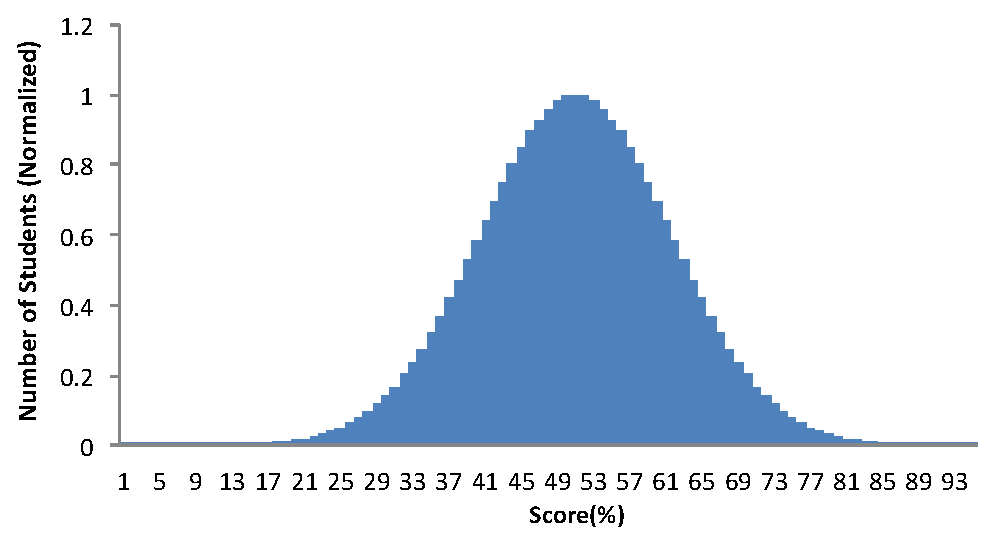
\includegraphics[scale=0.5]{Lab2_figs/hist_many.eps}
\end{center}

If we had infinitely many students, we would get a perfectly smooth curve.
You can see already that coloring in the bars in the graph is not useful any
more. So usually we just draw a point for the top of each bar. These points
form a curve.

\begin{center}
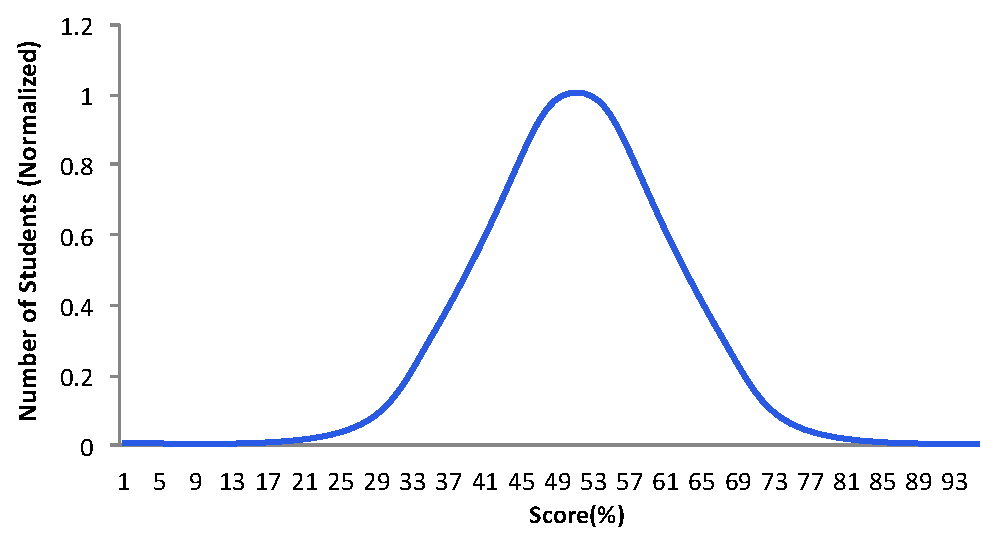
\includegraphics[scale=0.5]{Lab2_figs/hist_smooth.eps}
\end{center}

Unlike student scores, dart positions can be negative. So our dart
distribution should be centered on zero displacement. We will usually find
that $68\%$ of the darts will fall within $\pm \sigma $ of the mean. 

\begin{center}
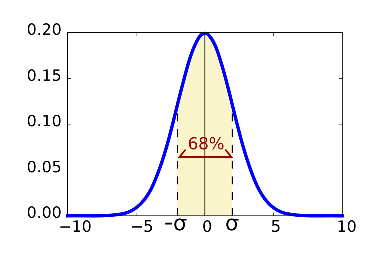
\includegraphics[scale=1.3]{Lab2_figs/normal_68.eps}
\end{center}

We can see that our $\sigma $ value is very like an uncertainty. But there
is a difference. We still have $32\%$ of our experiments outside of $\pm
\sigma ,$ and if we give the uncertainty, $\delta x,$ then all of the
measurements should be within $\pm \delta x.$ If you are building a space
shuttle and absolutely need to guarantee that your error on your calcuation
is within some limit, then you should use a true absolute uncertainty, $\pm
\delta x.$ But for most experiments, being that certain about our
uncertainty is not required, and we can use $\pm \sigma $ as a good
approximation to the uncertainty. We will often do this in this class. If
losing $32\%$ is not acceptable, but finding the true $\delta x$ is not
practical, it is often good enough to use $2\sigma $ or $3\sigma $ as the
estimate of our uncertainty. $95\%$ of the data will fall with $\pm 2\sigma
, $ and $99.7\%$ of the data will fall within $\pm 3\sigma .$ So these are
more conservative estimates than using a single standard deviation. But in
this class we will stick with just $\sigma .$

\section{Standard deviation of the mean}

Now you may wonder, does the mean value get better as we take more
measurements? That is, do we become more sure about where we are pointing if
we throw more darts and include these many darts' locations in our average?
I think you will see from our previous reasoning that this is the case. The
more trials of an experiment that we take, the closer our mean value is to
the \textquotedblleft truth\textquotedblright\ value we are measuring. Since
this is the case, shouldn't the uncertainty go down as we perform more
trials?

The answer is yes. We won't derive this in our class. But the estimate of
the uncertainty should be given by 
\[
\sigma _{\bar{x}}=\frac{\sigma _{x}}{\sqrt{N}} 
\]%
where $\sigma _{x}$ is our standard deviation in our $x$-position values and 
$N$ is the number of trials we took. The more trials that go into our
average, the lower our uncertainty estimate. The value $\sigma _{\bar{x}}$
is called the \emph{standard deviation of the mean}.

Notice that in some of our grade graphs, the most common score was not a $C.$
Here is an example: 

\begin{center}
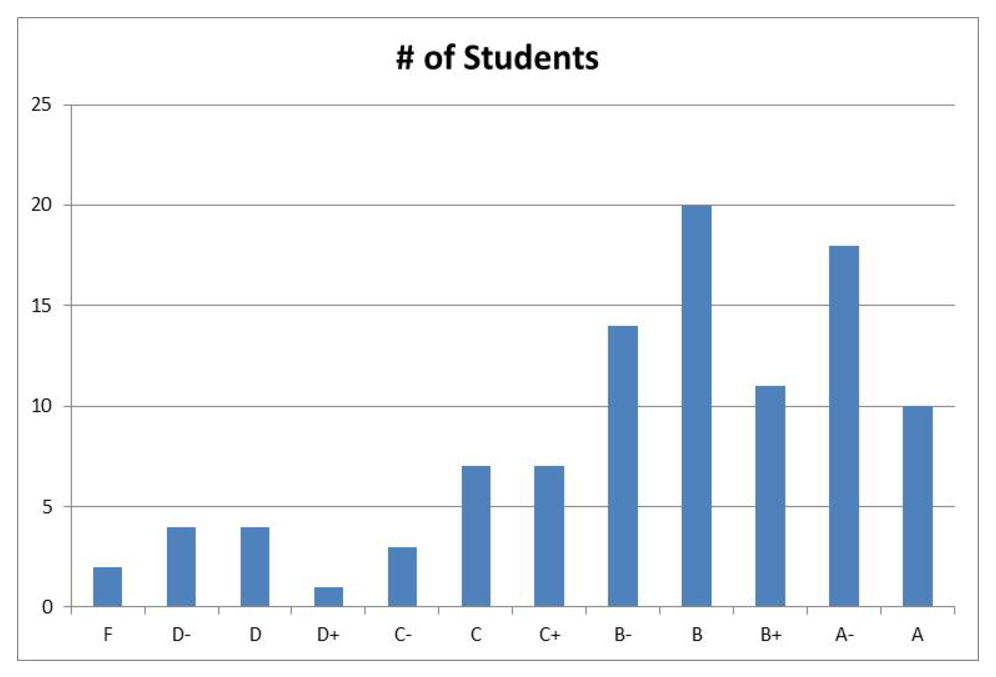
\includegraphics[scale=0.5]{Lab2_figs/hist_few.eps}
\end{center}

As students, this makes us all
happier, but for our error analysis this causes a problem. The error
analysis we have talked about so far assumes that our errors are distributed
in a very uniform way. If I go back to this graph

\begin{center}
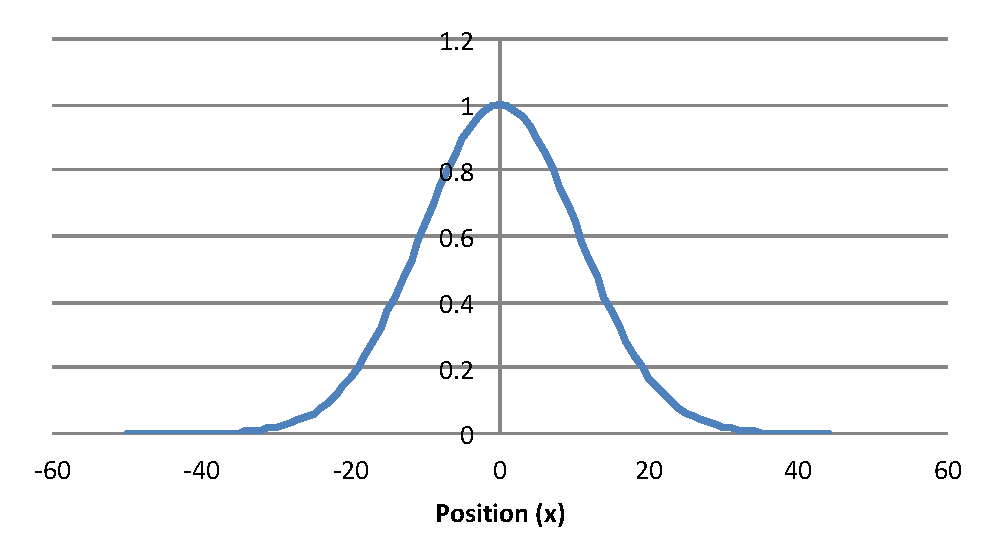
\includegraphics[scale=0.5]{Lab2_figs/hist_dart.eps}
\end{center}

we can see that there are as many
darts that landed to the left as there are to the right. This distribution
of errors is called the \emph{normal distribution}. Usually our errors in
our labs will be normally distributed. That makes all the math we talked
about work. But what if they are not, like our grade example? Well, that is
a great topic for PH336. So for now we will just assume a normal
distribution. But we can check to see how non-normal our data is. We can
find the \emph{mode} which is the value that occurs most frequently. For our
grade distribution above it would be a $B.$

We can also find the place where half of the trials landed on one side and
half on the other. This is called the \emph{median} point. We will calculate
both in our lab today. If we have a normal distribution, the average,
median, and the mode will all be the same. If this is not the case, then we
may worry a little about our error estimate--it may be too small.

\section{Graphical reporting of the mean (expected value) and standard
deviation (uncertainty)}

We now have a new view of measurement based on statistics. The mean value is
the value that we will say is our measurement. We call this the \emph{%
expected value}. The standard deviation is the representation of our
uncertainty. We can plot this in a way that communicates both at once. If we
take our eight data points that we started with earlier, we know the mean , $%
0.5\unit{cm},$ and we can find the standard deviation of the mean to be $0.6%
\unit{cm}.$ We plot this by making a dot or diamond or some larger point
indicator. Then we make a line through the point with little ends that show
the size of the uncertainty. The result looks like this.

\begin{center}
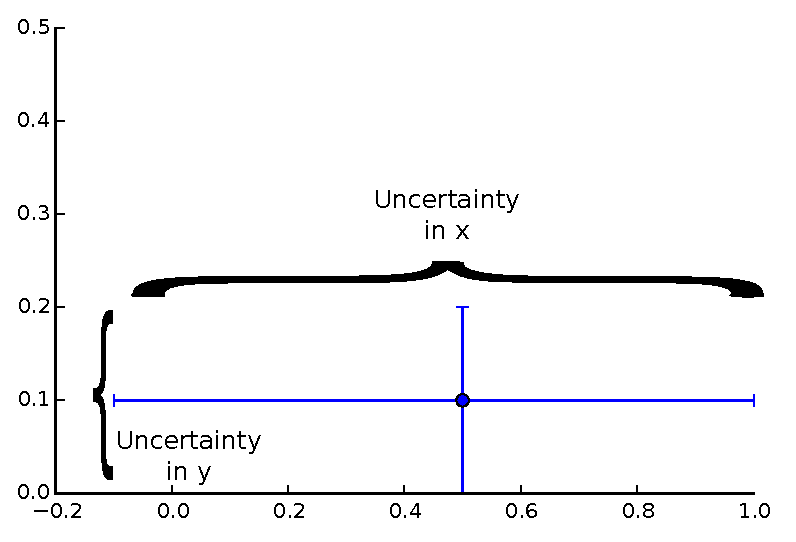
\includegraphics[scale=0.5]{Lab2_figs/error_bars.eps}
\end{center}

 Excel, and most plotting programs will allow you to
add error bars to your graphs.

Of course, we could have $y$
-direction error bars as well. These would be vertical, and there is no reason the $y$%
-error would be the same as the $x$-error. We may encounter such situations
in future labs.

\pagebreak

\section{Assignment}

Complete this lab in an organized fashion in your lab notebook. \emph{Part
of the grade will be based on neatness and organization!} There are several
histograms that need to be made during this lab. Make sure everyone in your
group gets a chance to build a histogram.

\subsection{Statistical Data I: How long does it take to walk?}

We will repeat one measurement, how long it takes to walk to a destination,
many times. Each person in our class will take the measurement once.

\begin{enumerate}
\item We'll start by determining a walking destination as a class. Our
destination is: \underline{\ \ \ \ \ \ \ \ \ \ \ \ \ \ \ \ \ \ \ \ }.

\item Each person in the class should get a digital timer and time their
walk to the destination and back. Walk at your normal walking speed. We will
stagger when you leave, to avoid walking in groups. While you are not
walking, you can begin working on part II.

\item When you return, record your walking time on the board to the nearest
second.

\item Record the times for all class members in a table
\item  \emph{by hand}
determine the mean walking time, the median walking time, and (if
appropriate) the modal walking time for the first 5 walkers. Determine the standard deviation of the
walking time of the first fve walkers\emph{by hand} (show all your work).

\item Using a computer: (see instructions below)
\begin{itemize}
\item 
\item confirm your mean walking time, median walking time, and (if appropriate) the modal walking time.
\item make a histogram of the walking times 
\end{itemize}
\end{enumerate}

\subsection{Making the Histogram in Python}
\subsubsection{Running your first Program}
Part of this class is learning to solve physics problems with a computer.  Today, you will be using the language python to find the median, and standard deviation of the walking data that we took.  Additionally, you will use it to make a histogram of the data.

When programming, it can be really helpful to make notes in your lab notebook about what each program does, things you learned about different functions, etc.  At the bare minimum you should include you final program, any graphs it makes, as well as where you saved it, and what name you saved it under.  That will make it easier to find in the future.

To begin writing your program, open up your favorite plain text editor.  I like notepad++ for windows or text wrangler on mac. Or, if you downloaded python from Enthought or Anaconda you can use Canopy (Enthought) or Spyder (Anaconda).   Enter the walking data like so: (Be sure to use the class data, not this sample data.)

\begin{lstlisting}[language=Python]
#Our walking data
data = [34, 38, 33, 38, 38, 36, 35, 47,36, 32, 40, 40, 
       45, 36, 43, 38, 48, 40, 40, 38, 43, 40, 39, 36, 46, 
       34, 37, 33, 32, 34 ]
print(data)

\end{lstlisting}
The first line is called a comment.  The |\#| tells the python interpreter (the thing that runs python) to ignore that line.  You should use comments to describe what your are doing in your program, that way you remember what it was later, or if anyone else has to read it they'll know what you did.  There will not be any more example comments in this tutorial.  You will have to come up with your own.

Let's look at the next set of lines:
\begin{lstlisting}[language=Python]
data = [34, 38, 33, 38, 38, 36, 35, 47,36, 32, 40, 40, 
       45, 36, 43, 38, 48, 40, 40, 38, 43, 40, 39, 36, 46, 
       34, 37, 33, 32, 34 ]
\end{lstlisting}
They load our walking data into what is called a list.  It's a way to save our data under a different name for easier access.
The |print(data)| command tells the computer to print out what we've saved in data.  

Save your file with the extension |.py|. (Example: |myFile.py|)  That tells your computer that it is a python script.

If you are using Canopy or Spyder, you can run your script by clicking play or hitting f5.  If you aren't using one of those, open up your command line on Windows or the terminal on Linux or Mac.  Navigate the where you saved your file (ask the instructor for help if you need it) and type in the command:
\begin{lstlisting}
python 'myFile.py'
\end{lstlisting}
but insert your file name. That tells your computer to run the python script.  You should see your data printed out on the screen.

\subsubsection{Finding the Mean, Median, and Standard deviation}

First, remove the |print(data)| line from your program. We don't need to have the computer spit that out again and again.  

Add these lines to your script:
\begin{lstlisting}[language=python]
import numpy as np
dataMean=np.sum(data)/len(data)
print('Mean:  {0:.2f}'.format(dataMean))
\end{lstlisting}

The first line loads a module called numpy.  Python keeps a lot of functions in separate modules.  Loading one is sort of like grabbing a book with the right set of instructions in it.  Now, all of the numpy functions are stored in the letters |np|.

The next line creates a variable called |dataMean|. The numpy sum command adds up all of the values in |data|, and |len(data)| gives you how many items are in the |data| list. (|len| is short for length).  

The third line prints |dataMean|.  Save your program again and run it to see what happens.  Try changing the 2 in the print command line to a three, save it, run it again, and see what has changed.

Numpy has a function that will calculate the mean for you.  Here's our script from above with one addition: |dataMeanNp| gives the mean of the data as calculated by numpy.
\begin{lstlisting}[language=python]
import numpy as np
dataMean=np.sum(data)/len(data)
print('Mean:  {0:.2f}'.format(dataMean))
dataMeanNp=np.mean(data)
print('Numpy Mean:  {0:.2f}'.format(dataMeanNp))
\end{lstlisting}


Your assignment for this part is to {\em add} these parts to your program:
\begin{enumerate}
\item a part where the program calculates and prints the standard deviation using the formula in the reading.
\item a part that uses numpy to find the median and standard deviation of our walking data.  The numpy function that finds the median is |median| and the numpy function that finds the standard deviation is |std|.
\end{enumerate}
Once you find the median and standard deviation, tell your script to print the median with no decimal places and to print the standard deviation to three decimal places. 

You should also include {\em comments} in your program.  Comments are notes for people to read, but that the computer will ignore.  You can start a comment with the |\#| character.  Part of keeping a good lab notebook is printing out copies of your programs, complete with comments. Here's the example program, all in one place, with good comments added:
\begin{lstlisting}[language=python]
#Load the class walking times into the variable "data"
data = [34, 38, 33, 38, 38, 36, 35, 47,36, 32, 40, 40, 
       45, 36, 43, 38, 48, 40, 40, 38, 43, 40, 39, 36, 46, 
       34, 37, 33, 32, 34 ]
       
#Importing the numpy library for easy calculations
import numpy as np

#Calculate the mean of data using the mean formula 
dataMean=np.sum(data)/len(data)
#Print the mean as a float with two decimal places
print('Mean:  {0:.2f}'.format(dataMean))

#Calculate the mean of the data using numpy's mean function
#If I did dataMean correctly, dataMeanNp should give the same result
dataMeanNp=np.mean(data)
#Print the mean calculated from numpy's function.  
print('Numpy Mean:  {0:.2f}'.format(dataMeanNp))
\end{lstlisting}

\subsubsection{Making a histogram}

Adding the following code to your script to make the histogram:

\begin{lstlisting}[language=python]
import matplotlib.pyplot as plt
plt.hist(data, 20, normed=0, facecolor='green', alpha=0.75)

plt.xlabel('My x axis Label')
plt.ylabel('My y axis label')
plt.title('My Title')
plt.savefig('myPlot.pdf')
\end{lstlisting}

This script will make a histogram with 20 bins and save it to the file |myPlot.pdf|.  In your program you should:
\begin{itemize}
\item Change the number of bins to something more appropriate for your data. If your fullest bin only has one or two items in it, you have way too man bins.  If everything fits into three or four bins, you have too few.  
\item Fix the plot title and axis labels to match what {\em you} are plotting. 
\item Add appropriate comments. If you have enough comments, it can be very helpful to refer back to this program in future weeks.  If you don't have enough, you will forget what this program does, and it won't be helpful to you.
\end{itemize}

Print out your completed program and histogram and add them to your lab notebook.
\end{document}

\documentclass{book}
\usepackage{amsfonts}
\usepackage{amsmath}
\usepackage{graphicx}
\usepackage{epstopdf}
\usepackage{amssymb}
\usepackage{hyperref}
\usepackage{textcomp}
\usepackage{listings}
\usepackage{units}
\usepackage{color}

\definecolor{dkgreen}{rgb}{0,0.6,0}
\definecolor{gray}{rgb}{0.5,0.5,0.5}
\definecolor{mauve}{rgb}{0.58,0,0.82}

\lstset{frame=tb,
  language=Python,
  aboveskip=3mm,
  belowskip=3mm,
  showstringspaces=false,
  columns=flexible,
  basicstyle={\small\ttfamily},
  numbers=none,
  numberstyle=\tiny\color{gray},
  keywordstyle=\color{blue},
  commentstyle=\color{dkgreen},
  stringstyle=\color{mauve},
  breaklines=true,
  breakatwhitespace=true,
  tabsize=3, upquote=true}

\lstMakeShortInline[columns=fixed]|

\setcounter{chapter}{2}

\begin{document}

\chapter{Measurement and Uncertainty II}

I\ hope that by now you have been taught what a derivative is in your Math 112
class. But if not, we will learn what it is today. For our purposes, a
derivative is a slope of a line. You should recognize the equation of a
straight line as
\[
y=mx+b
\]
The slope $m$ can be written as
\[
m=\frac{dy}{dx}
\]
This is nothing magic. It is just a strange way to write $m.$ With the slope
written this way, the equation of the line could be written as
\[
y=\frac{dy}{dx}x+b
\]
But why $dy/dx$? Think of how we find a slope of a line. Back in junior high
school we called the slope the \textquotedblleft rise over
run.\textquotedblright\ That is, the change in $y$-value divided by the change
in the $x$-value.
\[
m=\frac{y_{2}-y_{2}}{x_{2}-x_{1}}
\]
In physics, we write the change in a variable using the greek letter delta,
$\Delta.$ So we could write the slope as
\[
m=\frac{y_{2}-y_{2}}{x_{2}-x_{1}}=\frac{\Delta y}{\Delta x}
\]
\ We need to get used to this delta notation, so let me write out $\Delta y$
\[
\Delta y=y_{2}-y_{1}
\]
and $\Delta x.$
\[
\Delta x=x_{2}-x_{1}
\]
So our straight line equation should be written
\[
y=\frac{\Delta y}{\Delta x}x+b
\]
but if we take $\Delta x$ to be very, very small it is customary to write the
$\Delta x$ as just $dx$ (I guess a \textquotedblleft d\textquotedblright\ is
smaller than a \textquotedblleft$\Delta$\textquotedblright). If this is not
familiar from Math 112, is should be by now from PH121 (if is not familiar at
all, call me over for help, but still don't panic--we are just writing slope
in a strange way).

In PH121 you have or will shortly learn that the velocity is the slope of the
plot of $x$ vs. $t,$ for example,
\[
y=\frac{1}{2}\frac{\text{m}}{\text{s}}t+1\text{m}
\]
is an equation giving the $y$ position of an object as a function of time.
Note that it is a straight line on a $y$ vs. $t$ plot.
\begin{center}
\fbox{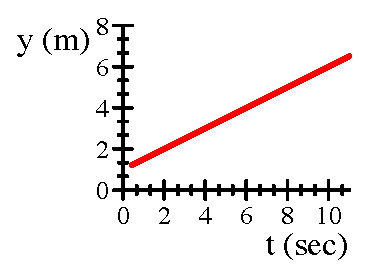
\includegraphics[
natheight=1.868000in,
natwidth=3.499900in,
height=1.868in,
width=3.4999in
]
{Lab3_figs/LineGraph.eps}
}
\end{center}
The slope of the line is
\[
\frac{dy}{dt}=\frac{1
\text{m}
}{2
\text{s}
}
\]
We can verify that this works by looking at the plot and noting that for every
two units of time, we go up one position unit. The slope is $1/2\frac{
\text{m}
}{
\text{s}
}.$

But not all curves are straight lines. What do we do with curves that, well, curve?

One idea is that we could split up the curve into little line segments, each
with its own slope. We can think of $dy/dt$ as an instantaneous slope, a slope
of one of the tiny line segments that make up our curve. This is the sort of
speed measurement that your speedometer gives. The speed might be different a
short time later. But right now the speed is, say, $0.5
\text{m}
/
\text{s}
.$

\begin{center}
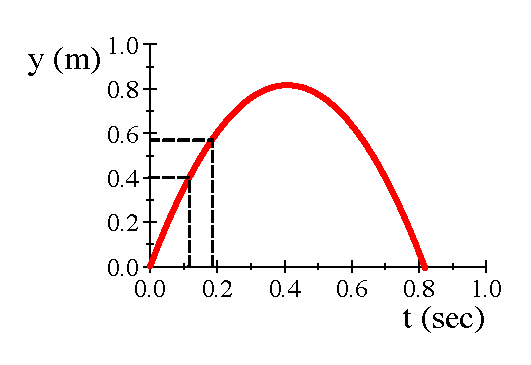
\includegraphics[
natheight=2.290000in,
natwidth=3.392700in,
height=2.3307in,
width=3.4385in
]
{Lab3_Figs/Parab_twopoints.eps}
\end{center}
Really, in defining an instantaneous slope we have assumed that the slope near
our point on the curve is essentially a straight line if $\Delta t$ is small enough.

We can use this idea to interpret our error calculations. Suppose I\ throw a
ball in the air with a initial speed of $4
\text{m}
/
\text{s}
$ straight up starting from $y_{o}=0$. From PH121 you have learned (or will
soon learn) that the equation for predicting how high the ball will go is
\[
y=y_{o}+v_{o}t+\frac{1}{2}at^{2}
\]
It says that starting at $y_{o}$ the ball will go higher depending on the
initial velocity, $v_{o},$ and the acceleration, $a.$ That make sense.

At a time, $t,$ the ball should be at
\[
y=0+4\frac{
\text{m}
}{
\text{s}
}t-\frac{1}{2}\left(  9.8\frac{
\text{m}
}{
\text{s}
^{2}}\right)  t^{2}
\]
where $a=-9.8\frac{
\text{m}
}{
\text{s}
^{2}}$ is the acceleration due to gravity. So, knowing this, I could predict
how high the ball would go if I\ pick a particular time, say, $0.15
\text{s}
.$ The result should be
\begin{align*}
y  & =0+4\frac{
\text{m}
}{
\text{s}
}\left(  0.15
\text{s}
\right)  -\frac{1}{2}\left(  9.8\frac{
\text{m}
}{
\text{s}
^{2}}\right)  \left(  0.15
\text{s}
\right)  ^{2}\\
& =0.489\,75
\text{m}
\end{align*}
This is shown in the next figure with a black line. Solving the equation for
$y$ is equivalent to drawing a line up to the curve, then from our spot on the
curve over to the $y$-axis to find the position.
\begin{center}
\fbox{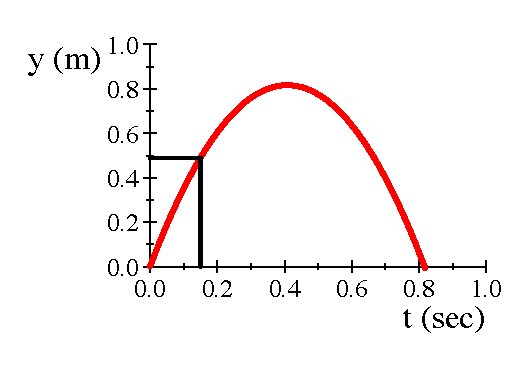
\includegraphics[
natheight=2.229500in,
natwidth=3.343400in,
height=2.2295in,
width=3.3434in
]
{Lab3_figs/Parab_onepoint.eps}
}
\end{center}


For our case we plot a line upward from $0.15
\text{s}
$ to the curve, and then plot a horizontal line from the intersection to the
$y$-axis. We can see that we get $4.9
\text{m}
.$ Suppose I try to verify this by taking a picture of the ball in flight at
$0.015
\text{s}
,$ but my stop watch is only good to $\pm0.005$ seconds. I try to take the
picture when the watch is at $0.015
\text{s}
,$ but I might have taken the picture at $0.01
\text{s}
$ or at $0.02
\text{s}
$ or anywhere in between. My time has some uncertainty. What does the
uncertainty in my stop watch time mean for the uncertainty in my $y$ value?

We can get a good approximation by graphically drawing vertical lines up from
$t_{\min}$ and $t_{\max}$ to the curve, and then extending horizontal lines
from the intersections to the $y$-axis. This gives us a $y_{\min}$ and
$y_{\max}.$ Our actual height could be anywhere in between these. This is a
way to view our uncertainty in $y.$
\begin{center}
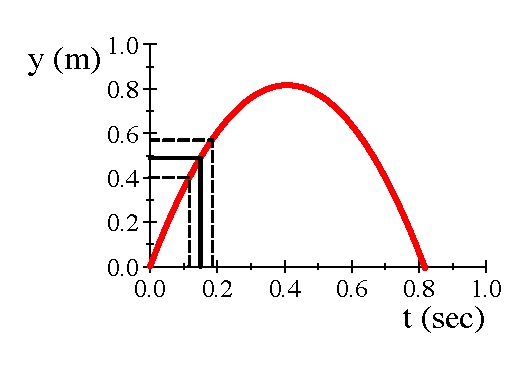
\includegraphics[
natheight=2.734500in,
natwidth=4.115600in,
height=2.7769in,
width=4.1658in
]
{Lab3_Figs/Parab_threepoints.eps}
\end{center}


We can use this idea to find a general way to calculate uncertainties. We
could define $\Delta t=t_{\max}-t_{\min}$. If our $\Delta t$ is small enough
(so we can write it just $dt$), the curve is essentially a straight line in
the region between $t_{\min}$ and $t_{\max}.$ So if we knew the slope of that
line (the derivative $dy/dt$) we could easily figure out the $y_{\max}$ and
$y_{\min}$ points to get our uncertainty range, at least if we stay near our
$t_{n}$ part of the curve. Recall that our uncertainty in $y $ using the
high/low method is
\[
\delta y=\frac{y_{\max}-y_{\min}}{2}=\frac{\Delta y}{2}
\]
Remembering that
\[
y=\frac{dy}{dt}t+b
\]
then
\begin{align*}
\Delta y  & =y_{\max}-y_{\min}\\
& =\frac{dy}{dt}t_{\max}+b-\frac{dy}{dt}t_{\min}-b\\
& =\frac{dy}{dt}\Delta t
\end{align*}
From your reading, you will recognize this as almost the uncertainty in a
function of one variable! But even if you don't recognize it, we can show that
this is true using our high/low method. The quantity $\Delta t$ is
\[
\Delta t=t_{\max}-t_{\min}
\]
so our uncertainty in $t$ would be
\[
\delta t=\frac{t_{\max}-t_{\min}}{2}=\frac{\Delta t}{2}
\]
then
\begin{align*}
\delta y  & =\frac{y_{\max}-y_{\min}}{2}\\
& =\frac{1}{2}\frac{dy}{dt}\Delta t\\
& =\frac{dy}{dt}\frac{\Delta t}{2}\\
& =\frac{dy}{dt}\delta t
\end{align*}
so
\[
\delta y=\frac{dy}{dt}\delta t
\]
So our uncertainty in $y$ is just the slope at our point on the curve
multiplied by our uncertainty in $t.$

But what if we have more than one variable? Say, we have a function $y(x,z),$
we essentially have a two dimensional slope. Think of a hill, you can go down
a hill in more than one direction. So we need slope parts for each direction
we can go.

But there is a fix we need to make to this equation that you won't learn for
several math classes to come. We want to have a slope in the $x$ and $z$
direction, but we want the slopes to be independent (if you have already taken
PH121, think of two dimensional motion problems, we split the problem into
components). The notation for this is
\[
\Delta y=\frac{\partial y}{\partial x}x+\frac{\partial y}{\partial z}z
\]
where
\[
\frac{\partial y}{\partial x}
\]
means the component of the slope just in the $x$ direction. We take a
derivative of the function $y,$ but assume only $x$ is a variable (treat $z$
and all $z$ terms with no $x^{\prime}s$ as constants). This lets us separate
the $x$ and $z$ parts. A special, one variable derivative like $\partial
y/\partial x$ is called a \emph{partial derivative} because you only take one
dimension of the derivative at a time. The reading from Chapter 3 uses this
type of derivative to find the general formula for error propagation. If we
wish to find the error in some general function $z\left(  x,y\right)  $ the
error is given by
\[
\delta y=\sqrt{\left(  \frac{\partial y}{\partial x}\right)  ^{2}\delta
x^{2}+\left(  \frac{\partial y}{\partial z}\right)  ^{2}\delta z^{2}}
\]
This looks a lot like our slope equation What we are doing is to assume the
function $y\left(  x,z\right)  $ is flat in a small region around the point we
are studying. then the function has a slope $\partial y/\partial x$ in the $x
$-direction, and $\partial y/\partial z$ in the $y$-direction. Each term like
\[
\left(  \frac{\partial y}{\partial x}\right)  \delta x
\]
gives how far off we could be in that direction (the $x$-direction in this
case). Remember that we have assumed that $y\left(  x,z\right)  $ is
essentially flat near our point of interest. The square root may be something
of a mystery, but remember what you have learned or are learning about adding
vectors in PH121. We add components of a vector to find the magnitude like
this
\[
V=\sqrt{V_{x}^{2}+V_{y}^{2}}
\]
This comes from the Pythagorean theorem. The $x$ and $y$ parts of the vector
form two sides of a triangle. We want the remaining side. So we use the
Pythagorean theorem to find the length of the remaining side.

We are doing the same for our small uncertainty lengths. We are just adding
the $x$ and the $y$ components of the error. We could write our error formula
for the general case of a function $f$, that depends on $N$ different
variables.
\[
\delta f=\sqrt{\sum_{i=1}^{N}\left(  \frac{\partial f}{\partial x_{i}}\right)
^{2}\delta x_{i}^{2}}
\]
We will use this formula a lot, so make sure you understand what it means (ask
your instructor for help if it is not clear).

\section{How do we find the slope?}

But now we have an equation in terms of slope written as $dy/dx$ or $dy/dz$,
but how would we ever find these slops? Your calculus class has or will teach
you this. So we will just give you some quick formulas that will work for most
equations, then you can ask your instructor if you have something odd like an
$\arctan$ function.

For polynomials like,
\[
f\left(  x\right)  =ax^{2}+bx+c
\]
each term follows the rule
\[
\frac{d}{dx}\left(  ax^{n}\right)  =anx^{n-1}
\]
that is, if I have a constant, $a,$ times $x^{n}$ the slope of this curve is
the constant, $a,$ times the power, $n,$ times $x$ to the $n-1$ power.

Let's take an example. What is the slope of the function $y=5x^{3}?$

\[
\frac{d}{dx}\left(  5x^{3}\right)  =\left(  5\right)  \left(  3\right)
x^{3-1}=15x^{2}
\]


How about finding the slope of $y=7x^{2}-2x+1$

\[
\frac{d}{dx}\left(  7x^{2}-2x+1\right)  =\left(  7\right)  \left(  2\right)
x^{1}-\left(  2\right)  (1)x^{0}+0
\]
The last term illustrates that the slope of a constant is zero. That makes
sense. Constants don't change. So the change in $y$ just due to the last term
$(1)$ should be zero. We also remember $x^{0}=1.$ So we are left with
\[
\frac{d}{dx}\left(  7x^{2}-2x+1\right)  =14x-2
\]


This one rule will take care of most of our functions for now. Let's try one
more, say $y=x^{\frac{1}{2}}$
\[
\frac{d}{dx}\left(  x^{\frac{1}{2}}\right)  =\frac{1}{2}x^{-\frac{1}{2}}
\]
This could be written as
\[
\frac{d}{dx}\left(  \sqrt{x}\right)  =\frac{1}{2}\frac{1}{\sqrt{x}}
\]
So we see we can handle square roots with this rule.

\section{Tie to statistics}

We need to tie our statistical ideas into what we have learned about error
propagation. Lets go back to our function $f\left(  x,y\right)  $ the error is
given by
\[
\delta f=\sqrt{\left(  \frac{\partial f}{\partial x}\right)  ^{2}\delta
x^{2}+\left(  \frac{\partial f}{\partial z}\right)  ^{2}\delta z^{2}}
\]
but now we know we could express this in terms of standard deviations
(provided you don't need to ensure all data are within your uncertainty
range). We can write our uncertainties as
\[
\sigma_{f}=\sqrt{\left(  \frac{\partial f}{\partial x}\right)  ^{2}\sigma
_{x}^{2}+\left(  \frac{\partial f}{\partial z}\right)  ^{2}\sigma_{z}^{2}}
\]


We can use this to show that the standard deviation of the mean (the best
estimate of our uncertainty) is given by

\[
\sigma_{\bar{x}}=\frac{\sigma_{x}}{\sqrt{N}}
\]
Think of calculating a mean value
\[
\bar{x}=\frac{x_{1}+x_{2}+\cdots x_{N}}{N}
\]
We can find the uncertainty in this function $\sigma_{\bar{x}}$
\[
\sigma_{\bar{x}}=\sqrt{\left(  \frac{\partial\bar{x}}{\partial x_{1}}\right)
^{2}\sigma_{x_{1}}^{2}+\left(  \frac{\partial\bar{x}}{\partial x_{2}}\right)
^{2}\sigma_{x_{2}}^{2}+\cdots+\left(  \frac{\partial\bar{x}}{\partial x_{N}
}\right)  ^{2}\sigma_{x_{N}}^{2}}
\]
You see we just take the partial derivative of our function $\bar{x}$ with
respect to each of the variables $x_{i}$ and multiply by the uncertainty in
that variable written now as a standard deviation $\sigma_{i}.$

For this special case, all of the $x_{i}$ are the same (we are measuring the
same value over and over in taking an average) and all of the $\sigma_{i}$ are
the same so we just have
\[
\sigma_{\bar{x}}=\sqrt{N\left(  \frac{\partial\bar{x}}{\partial x_{1}}\right)
^{2}\sigma_{x_{1}}^{2}}
\]
and we can take the derivative using our rule. Only $x_{1}$ is a variable, so
we can write the average $\bar{x}$ as
\[
\bar{x}=\frac{x_{1}}{N}+\frac{x_{2}+\cdots x_{N}}{N}
\]
This is a polynomial! The first term is $\frac{1}{N}x_{1}$ and the whole
second term is a constant if we take a partial derivitive with respect to
$x_{1}$. The derivative is
\begin{align*}
\frac{\partial\bar{x}}{\partial x_{1}}  & =\frac{\partial}{\partial x_{1}
}\left(  \frac{x_{1}+x_{2}+\cdots x_{N}}{N}\right) \\
& =\frac{1}{N}x_{1}^{0}+0\\
& =\frac{1}{N}
\end{align*}
so our statistical error function is just
\begin{align*}
\sigma_{\bar{x}}  & =\sqrt{N\left(  \frac{1}{N}\right)  ^{2}\sigma_{x_{1}}
^{2}}\\
& =\sqrt{\frac{\sigma_{x_{1}}^{2}}{N}}\\
& =\frac{\sigma_{x_{1}}}{\sqrt{N}}
\end{align*}
or, since all the $\sigma_{x_{i}}$ are the same, we can just write this as
\[
\sigma_{\bar{x}}=\frac{\sigma_{x}}{\sqrt{N}}
\]


Notice that in this example we had many $x_{i}$ and that to find the
uncertainty we just extended our equation from two variables
\[
\sigma_{f}=\sqrt{\left(  \frac{\partial f}{\partial x}\right)  ^{2}\sigma
_{x}^{2}+\left(  \frac{\partial f}{\partial z}\right)  ^{2}\sigma_{z}^{2}}
\]
to $N$ variables
\[
\sigma_{f}=\sqrt{\sum_{i=1}^{N}\left(  \frac{\partial f}{\partial x_{i}
}\right)  ^{2}\sigma_{i}^{2}}
\]


In this special case, we were trying to show a special result, but we can do
this for any function with any number of variables. If your function is
complicated, you just need to take more partial derivative terms under the
square root.

\pagebreak

\section{Assignment}

Measure the acceleration due to gravity, $g,$ four different ways. For each
case, determine an experimental value for $g$ along with its uncertainty.
Record how you find $g$ and its uncertainty for each method in your lab
notebook. Try to obtain the best value you can for each method.

\subsection{Method 1: Timing a ball drop}

Using a stop watch and a tennis ball, drop the ball over a known height and
determine a value for $g.$

\subsection{Method 2: Using a pendulum}

You will learn in PH123 that a pendulum oscillates back and forth at a certain
rate. If you don't plan to take PH123, you still know that the pendulum of a
grandfather clock sets the rate at which the clock will run. The time it takes
the pendulum to go back and forth is called the \emph{period of oscillation}.
That period is given by the following equation
\[
T=2\pi\sqrt{\frac{L}{g}}
\]
where for some reason the letter $T$ stands for period, and $L$ is the length
of the pendulum string, and $g$ is the acceleration due to gravity. Build your
pendulum, and measure the period of oscillation using a photogate. From this
obtain a value for $g.$

\subsection{Plot Your Results}

A spreadsheet program (e.g. MS Excel or LibreCalc) can graph data, and so can
a piece of software on our lab computers named LoggerPro. You may know how to
make a graph in one of these tools.

In this class, we are using python, so you should try making your plot in python.  Last week, we used matplotlib to build a histogram. The command for building a plot with errorbars is very similar.  Assuming that you've imported matplotlib as |plt|, the command looks like this:
\begin{lstlisting}[language=python]
plt.errorbar(x,y,xerr=xerr_variable,yerr=yerr_variable,fmt='o')
\end{lstlisting}
|xerr| and |yerr| are optional commands. If you you want error bars in the x direction, and you've saved the size of your x error in the variable |my_x_err|, sometime after your x and y lists, you'd include the command |xerr=my_x_err|. If you don't have any x-error bars, leave out |xerr|.

  Try to make a plot of the two different values you found for $g$, with errorbars, by using the |errorbar| command and by borrowing and adapting parts of last week's program. The commands for labeling the axes, title, etc. for an |errorbar| plot are the same as the commands for a histogram.

\subsection{Method 3: High Speed Camera}

Take high speed video of a falling ball. Important things to do as you take your video:
\begin{itemize}
\item Include a meter stick or something of known length in your video. 
\item Try not to move the camera as you take the video
\item If you record with high speed on a cell phone, make sure that the frame rate is constant.  Many smart phones will let you start in real time, slow it down, then speed it up again.  Do not do this.
\end{itemize}




Use either the \emph{Logger Pro} or \emph{Tracker} software to analyze the
video. Tracker has an autotracking option that can be very helpful if your ball does not blend into the background of your video. The steps to do this in Logger Pro are outlined in the Logger Pro help under
``video analysis."  The steps to do this in Tracker are on their web page under video tutorials.  ``Tracker Quick Start" gives a short version (2.5 min.). ``Getting Started with Tracker" has a longer version.

Fit a curve to your data that comes from the video. From you PH121 experience
you know that the acceleration due to gravity is constant, so we can use the
equation
\[
y=y_{o}+v_{o}t+\frac{1}{2}at^{2}
\]
to indicate the type of curve to use for our fit. If you have trouble finding
the curve fit function in Logger Pro or Tracker, or have trouble using Logger Pro or Tracker, call
your instructor over.




\end{document}

\documentclass[twoside,11pt,ShortChapTitles]{BYUTextbook}

\usepackage{soul}
\renewcommand{\vec}[1]{\ensuremath{\mathbf{#1}}}
\usepackage{siunitx}
\sisetup{round-mode = figures,
  round-precision = 3, scientific-notation=true}
  \usepackage{marginfix}

\usepackage{mathtools}






\setcounter{chapter}{3}
\renewcommand{\chaptername}{Lab}
\begin{document}


\chapter[Experimental Design I]{Experimental Design I: Harmonic Oscillators (masses and springs)\label{Experimental Design}}


This week's assignment follows the experimental design process outlined in the introduction to the lab.  We are trying to determine whether or not
I have mostly designed this experiment for you. So this week I want you to
identify the design parts and put them in our design process order. For our
next design lab, you will have to design the experiment yourself. This week's
lab is to get familiar with the process. Perform this experiment as a group.

\section{First Part: Data Collection}

\begin{enumerate}
\item Our system will be the mass-spring system and it's hanger. Obtain a set
of weights, a spring, a weight hanger, a stand, and a stopwatch. Attach the
spring to the stand, and the weight hanger to the spring. Determine the inputs
to this mass-spring system that may affect the output quantity of interest
(the period of oscillation). Determine whether each of these inputs will
affect the period of oscillation. If so, explain how you will control for that
input. If not, give justification for why you can ignore that input.

\item Build a mathematical model beginning with the suggestion you got from
reading Hook's work (lab introduction).

\item Determine how you will measure the period of oscillation. Remember that
you want to minimize the amount of uncertainty in your measurement. Techniques
we have learned in previous labs may help. Record your method. You should plan
any graphs you will make and in general plan how you will report your data and
whether or not your experiment is successful.

\item Discuss how you might go about making your equation look linear by a
proper substitution of variables. Explain why this might be useful.

\item Select a range of variables. (e.g. $m=$ $20
\operatorname{g}
$, $30
\operatorname{g}
$, $40
\operatorname{g}
$, $50
\operatorname{g}
$, and $100
\operatorname{g}
$). Don't use $80
\operatorname{g}
$ because I want to reserve this value for a special purpose below. Stop at
about $100
\operatorname{g}
.$

\item Plan your procedure and record your plan in your lab notebook.

\item Perform the experiment. Your plan probably includes determining the
period of oscillation for masses that you have selected. Be sure to record any
measurement uncertainty. Make the graphs of your data that you planned
including the appropriate error bars and a best fit line (See second part). Attach the graphs in your lab notebook.
Record what you do and highlight any deviations from your planned procedure.
Record your data or your data file name and location. Show your analysis and
give your results. Draw conclusions. We will check these conclusions in the
third part. But state whether you believe that $T\propto\sqrt{m}$
\end{enumerate}

\section{Second Part: fitting a line}
In order to fit a line to your data, you'll need to teach Python how to do a linear least squares fit using the equations and the example function in the lab introduction.  You will be doing many linear least squares fits, so it is in your best interest to create a least squares function in its own file that you can use in the future.  That way you don't have to copy and paste it over and over again. These steps will teach you how.
\begin{enumerate}
\item Linearize your equation.  Remember, linear least squares fitting only works on lines.
\item Type out the example program given in this lab's intro, and save it in the folder where you have been saving your other programs from lab.  Make sure that you match the indentation from the example.  Python uses indentation to tell where functions end.  Here's a quick example:
\begin{lstlisting}
def line(x,m,b):
    return m*x+b

\end{lstlisting}

Notice the difference in indentation between the two lines. The "def" command tells Python that you want to create your own function.  In this case, the function is called \code{line} and takes inputs \code{x}\sidenote{This function assumes that \code{x} is a numpy array.  If it is a regular list, the multiplication won't work the way you expect it to.},\code{m}, and \code{b}.  The return command tells Python what you want to get out of your function.  You could define a function this way and get the same result:

\begin{lstlisting}
def line(x,m,b):
    y=m*x+b
    return y

\end{lstlisting}

But you will get an error if you enter this:
\begin{lstlisting}
def line(x,m,b):
    y=m*x+b
return y

\end{lstlisting}
Indentation is very important in Python.  When you define a function, everything that is indented below it is counted as part of that function.  Not indenting the return statement tells Python that you've ended your function, and it won't know what to return.
Here's one more example:
\begin{lstlisting}
def line(x,m,b):
    y=m*x+b
    return y

y=line(5,2,1)

\end{lstlisting}
The previous piece of code tells Python what we want our function to be.  Then,  the very last line (notice that it is not indented) tells Python that we want to use our function, and that we want \code{x=5}, \code{m=2}, and \code{b=1}.  Python will perform the operation and save the number 11 (the result of 5*2+1) into the variable \code{y}.  Python will also treat any variables inside of functions as separate from the ones outside, meaning the \code{y} in our function is independent of the \code{y} in the last line. Once you define a function, you can use it over and over again in your program.

\item Test your function.  Put these lines of code {\em after} your function\sidenote{The \code{if __name__ == "__main__":} line tells Python to only run this part of the program when you are running this particular file.  If you leave it out, Python will run this test whenever you load your function into another file.}:
\begin{lstlisting}
if __name__ == "__main__":
    xdata=[1,2,3,4,5,6]
    ydata=[1,2,3,4,5,6]

    #Run linear least squares fit on the data
    slope, intercept = linear_least_squares(xdata,ydata)

    #Print out the test values
    print('Slope: {}'.format(slope))
    print('Intercept: {}'.format(intercept))

\end{lstlisting}
If your program is working properly, it will print:
\begin{lstlisting}
Slope: 1.0
Intercept: 0.0

\end{lstlisting}

\item It is also very important to be able to calculate error.  Modify the \code{linear_least_squares} function so that it also returns the error in the slope ($\sigma_m$) and intercept ($\sigma_b$).  As a reminder, these equations calculate the error:
\[\sigma_m=\frac{\sigma_y}{\sqrt{N\left(\left<x^2\right>-\left<x\right>^2\right)}}\]
\[\sigma_b=\sigma_y\sqrt{\frac{\left<x^2\right>}{N\left(\left<x^2\right>-\left<x\right>^2\right)}}\]
where
\[\sigma_y=\sqrt{\frac{1}{N-2}\sum_i^N \left(y_i-b-mx_i\right)^2}\]

The error in both the slope and intercept should be zero if your fit is working properly.
\end{enumerate}

Now start building a script to fit this week's data.
\begin{enumerate}
\item Open up a new Python script and save it in the same directory as your least squares file.  Put this command at the top of your file: (For this example, the file with the least squares fitting functions in it was saved with the name \code{linear_least_squares.py}, change the name to match accordingly.)
\begin{lstlisting}
import linear_least_squares

\end{lstlisting}
This line tells Python to load all of the functions in \code{linear_least_squares.py}.  You can now use your least squares fitting function in this program.

\item Load your data into your program. Doing math with data sets is easier in Python if you use the numpy library.  It can be very helpful to save our data like this\sidenote{It would be good to give your data more descriptive names than \code{x_data} and \code{y_data}, and add comments.}:
\begin{lstlisting}
import numpy as np
x_data=np.asarray([1,2,3,4,5])
y_data=np.asarray([2.1, 3.9, 5.8, 8.4, 11])

\end{lstlisting}
As an experiment, tell Python to \code{print(x_data*y_data)} and see what happens.    Numpy arrays can only have numbers in them, and so multiplying two numpy arrays will multiply each item in the list individually.  Since Python lists can have anything in them (numbers, words, other lists) Python doesn't have a built in way to do math on entire lists without doing quite a bit more work.  That's mostly because it doesn't make any sense to say \code{5*'hello'}.

\item Do a least squares fit to your data using your fitting functions.

\item Check your fit equation by using your fitted slope and intercept to
calculate a new set of \code{y} values (\code{yfit=m*x+b}) and then plotting them. (Data points with errorbars, as well as the fit line) The \code{matplotlib.pyplot} command for plotting a regular line is \code{plot(x_points,y_points)}.


\end{enumerate}

\section{Third Part: Interpolation and Extrapolation}

We would like to test the equation or  ``law" you developed in the last part. We will use the equation to predict periods
for masses you have not yet used.

\begin{enumerate}
\item \textbf{By interpolation, predict the period of oscillation for an }$80
\operatorname{g}
$\textbf{\ mass.} Record your methods and results. Interpolation means to
predict an output value (in this case, a period) for an input value that falls
within the range of the input values you have used in your measurements. If
you measured periods for $20
\operatorname{g}
$, $30
\operatorname{g}
$, $40
\operatorname{g}
$, $50
\operatorname{g}
$, and $100
\operatorname{g}
,$ then $80
\operatorname{g}
$ is within this range. Using the curve fit equation generated by the data we
measured, we can plug in $80
\operatorname{g}
$ and predict the period for our spring with an $80
\operatorname{g}
$ mass. This is interpolation. This will test our model to see if it works for
new inputs. If it does not, our model is probably not good.

\item \textbf{By extrapolation, predict the period of oscillation for a }$300
\operatorname{g}
$\textbf{\ mass.} Record your methods and results. Extrapolation means to
predict an output value (in this case, a period) for an input value that falls
outside the range of the input values you have previously measured. If you
measured periods for $20
\operatorname{g}
$, $30
\operatorname{g}
$, $40
\operatorname{g}
$, $50
\operatorname{g}
$, and $100
\operatorname{g}
,$ then $300
\operatorname{g}
$ is outside this range. Using the curve fit equation generated by the data we
measured, we can input $300
\operatorname{g}
$ and predict the period for our spring with an $300
\operatorname{g}
$ mass. Extrapolation is more risky. The conditions of our experiment might
change outside our range (think, in a limiting case, we could break the
spring, and get an infinite period!). But if things are done carefully, this
is also a test of the validity of our model.

\item Measure the period of oscillation for the $80
\operatorname{g}
$ and $300
\operatorname{g}
$ masses. Be sure to account for all uncertainties. Compare your measurements
with your predictions, and comment on the level of agreement.

\item Now that we have tested our mathematical model for the relationship
between period and mass for a mass-spring system, you can report it. Determine
values for your constants, including uncertainties . Record your methods and results.
\end{enumerate}

\subsection{Third Part: Further Discussion}

\begin{enumerate}
\item An often useful tool, especially when your data is not naturally linear,
is to plot it on a logarithmic scale. Create such a graph using Python and attach it to your lab notebook.  The matplotlib function is \code{semilogy(x\_data,y\_data)}. Comment on what you see.

\item Don't forget to make good comments on what you did and how you did it in
your lab book.
\end{enumerate}

\end{document}

\documentclass[twoside,11pt,ShortChapTitles]{BYUTextbook}

\usepackage{soul}
\renewcommand{\vec}[1]{\ensuremath{\mathbf{#1}}}
\usepackage{siunitx}
\sisetup{round-mode = figures,
  round-precision = 3, scientific-notation=true}
  \usepackage{marginfix}

\usepackage{mathtools}






\setcounter{chapter}{4}

\begin{document}
\chapter{Experimental Design II: Conservation of Energy}

This week we will practice experimental design with a new context. I wont
spell out all the steps, so your lab group and you will have to work through
the experimental design steps.

Suppose you have been told that energy is conserved (I\ hope you have by now
in PH121). This is our model--the idea that energy is conserved. That is,
that it is never lost, just transferred from one form of energy to another.
A colleague suggests a method to test this model. He builds a pine-wood
derby track and a pinewood derby car.
\begin{center}
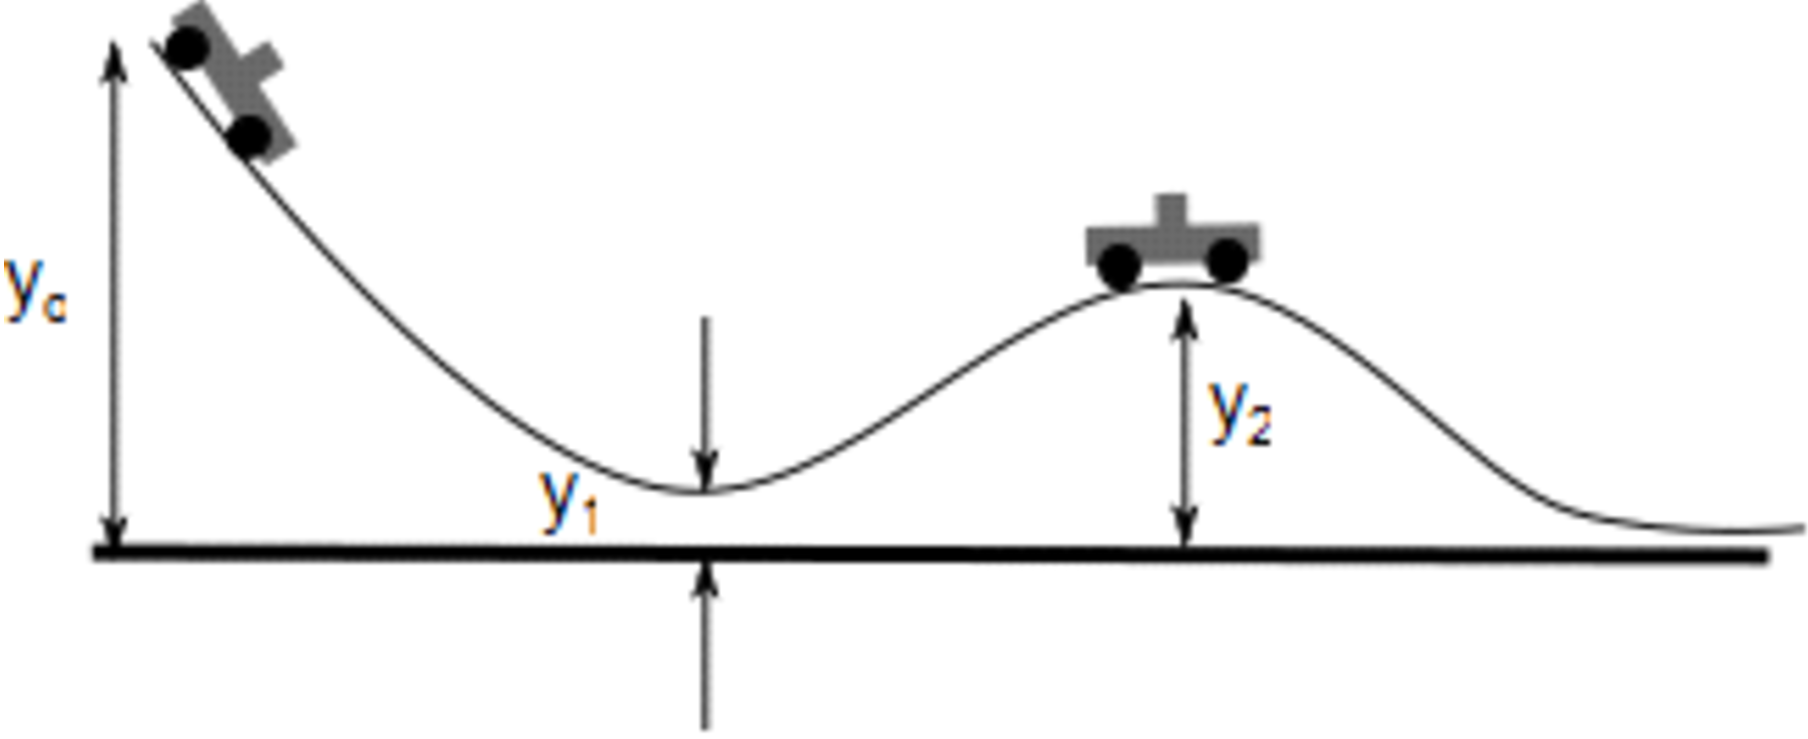
\includegraphics[width=0.5\textwidth]{Lab5_figs/LHDZMM03.png}
\end{center}
Your colleague suggests to you
that if energy is conserved, you should be able to predict the velocity of
the car at points $y_{1}$ and $y_{2}.$

Another colleague steps in and suggests that you need to be concerned about
the energy tied up in the rotational kinetic energy of the wheels. You may
not have heard about this in your PH121 class yet. She says that is OK,
because you can do a quick fix. She suggests that you should include a
factor of about 10\% of the translation kinetic energy. That is, compute the
kinetic energy in this case as%
\[
K=\left( 1.1\right) \frac{1}{2}mv^{2} 
\]%
that should account for the wheel rotational kinetic energy.

\pagebreak

\section{Assignment}

\subsection{Part 1:}

As a group design an experiment to test the model. Your design should
include the steps from lab \ref{Experimental Design} (briefly repeated here)

\begin{enumerate}
\item Identify the system to be examined. Identify the inputs and outputs.
Describe your system in your lab notebook.

\item Identify the model to be tested. Express the model in terms of an
equation representing a prediction of the measurement you will make. Record
this in your lab notebook. (If you have not solved this problem in your
PH121 class yet, call me over and we will go through it together).

\item Plan how you will know if you are successful in your experiment. Plan
graphs or other reporting devices. Record this in your lab notebook. For
today's lab, I\ will provide photogates and the car and track. If you need
other equipment, ask.

\item Rectify your equation if needed. Record this in your lab notebook.

\item Choose ranges of the variables. Record this in your lab notebook.

\item Plan the experimental procedure. Record this in your lab notebook.

\item Perform the experiment. Record this in your lab notebook. Go through
all the steps of performing an experiment. End with a conclusion that
clearly states whether your experiment supported the model, falsified the
model, or, if neither was possible, try to explain why.
\end{enumerate}

\subsection{Part 2}

Work on your proposals. They are due in two weeks. Here are some tips on
writing your proposal:

\subsubsection{Proposal writing:}

A Proposal is a document that is intended to persuade someone (your
professor, funding agency, yourself, etc.) that you should be given the
resources and support to perform the experiment. For our class, the proposal
consists of the following parts:

\begin{enumerate}
\item Statement of the experimental problem

\item Procedures and anticipated difficulties

\item Proposed analysis and expected results

\item Preliminary List of equipment needed
\end{enumerate}

Note that most of the steps involved in planning an experiment are contained
in these for parts of the proposal. Each of the steps is explained in more
detail below.

\paragraph{\textbf{Statement of the experimental problem:}}

This is a physics class, so our experiment should be a physics experiment.
The job of an experimental physicist is to test physics models. So your
statement of the experimental problem should include what model you are
testing and a brief, high level, overview of what you plan to do to test
this model.

\paragraph{\textbf{Procedures and anticipated difficulties:}}

Hopefully, your reader will be so excited by the thought of you solving your
experimental problem that he or she will want to know the details of what
you plan to do. You should describe in some detail what you are planning. If
there are hard parts of the procedure, tell how you plan to get through
them. This is essentially steps 1-6 of our experimental design strategy.

\paragraph{\textbf{Proposed analysis and expected results:}}

You might think this is unfair, how are you supposed to know what analysis
will be needed and what the results should be until you take the data? But
really you both can, and should make a good plan for your data analysis and
figure out what your expected results should be before you start taking
data. After all, you have a model you are testing. You can encapsulate that
model into a predictive equation for your experiment. Then you can use that
predictive equation to obtain predicted results and uncertainties. Using
this, you can design your experimental apparatus by putting in the numbers
from your experimental design and seeing what the outcome should be. You can
see if there is a chance that your experiment will measure what you want
with the equipment you have (this is where our differential form of error
calculation comes in).

If you don't do this, you don't know what equipment you will need or how
sensitive that equipment needs to be. If you are trying to measure the size
of your text book, an odometer that only measures in whole miles may not be
the best choice of equipment. This might be obvious, but depending on how
well you need to measure your text book, a ruler may not work either. You
don't know until you have an estimate of the uncertainty. So to know what
you need, do the calculations in advance with your range of inputs as the
values you take for the prediction.

Of course this means you must include a predictive calculation of the
uncertainty. Uncertainty in your result is governed by the uncertainty
inherent in the measurements you will take. The uncertainty calculation
tells you what sensitivity you will need in your measurement devices. In our
text book case, you could see immediately that you need a different
apparatus than the odometer. You might also find our ruler to be problematic
depending on what precision you need.

I remember a time in my career when the US\ Naval Research Labs asked us to
build a microwave radiometer to measure the sea wind direction from space.
We spent some time and our predicted analysis and uncertainty said that it
would be a very expensive instrument to be able to successfully measure the
wind direction---it would take more money than they were offering. NRL
disagreed and built the device themselves at less cost, but to lesser
specifications with much greater uncertainties. Then they spent a billion
(yes, a billion with a \textquotedblleft b\textquotedblright ) dollars to
launch the device into space. The device was a total failure. The
uncertainty was so big that the data was totally useless. We want to find
out whether our experiment will work before we risk our grades (or a billion
dollars) on it. So we will do the prediction ahead of taking the data.

You should do all of this symbolically if you can, numerically if you must,
but almost never by hand giving single value results. Some measurements will
come back poorer than you anticipated, or some piece of equipment will be
unavailable. You don't want to have to redo all your calculations from
scratch each time this happens. For example, in the event of an equipment
problem, your analysis tells you if another piece of equipment is
sufficiently sensitive, or if you need to find an exact replacement. When I\
perform an analysis like this, I try for a symbolic equation for
uncertainty. I\ like to program these equations into Scientific Workplace,
or Maple, or SAGE, or MathCAD, or Mathmatica or whatever symbolic math
processor I\ have. Then, as actual measurements change, I\ instantly get new
predictions. In the absence of a symbolic package, a spreadsheet program
will do fine (and we have Excel on our computers). A numerical program also
is quick and easy to re-run with new numbers when no symbolic answer is
found.

\subsubsection{Preliminary List of equipment needed}

Once you have done your analysis, you are ready to list the equipment you
need and the sensitivity of the equipment you need (that is, list the
uncertainties you need to achieve). Final approval of the project and the
ultimate success of your experiment depends on the equipment you choose or
are granted. You want to do a good job analyzing so you know what you need,
and a good job describing the experiment so you are likely to have the
equipment you want available when you start.

\subsubsection{Performing the experiment}

Once your proposal is accepted, I\ will provide you with the equipment we
have agreed upon from your proposal. You will have three weeks to perform
your experimentation. I\ will be available for advice and to watch for
problems or safety issues. But you and your team will perform the
experiment. \textbf{You will want to keep good notes in your lab notebook.}
You will likely have to change your procedure after you start because of
problems. Take careful note of what was actually done, and what your
measurements were. Give the reason for the change. Note any unusual things
that happen. \textbf{Carefully record what you do.}

\subsubsection{Written report}

The written report is designed to match a normal format for an applied
physics article in a journal like \emph{Applied Optics} or the \emph{IEEE
Transactions} journals.\emph{\ }It is useful to know now how I\ will grade
the report later so you can make sure you design in all the parts I will
look for. There should be an introduction, description of the procedure,
description of the data and results, a description of the analysis, and a
conclusion. These sections are described in detail in the following table.

Experimentation is a lot of fun if done right. It can be frustrating and
discouraging if not done well. Our goal is to learn how to perform and
report on an experiment, so that is what will be graded. If you show
something new and interesting, that is just more fun. If you show that your
original model was not correct--that is science! If you have done a good job
designing and reporting your experiment, a negative result is just as good
as a positive result.




\end{document}
\documentclass{book}
\usepackage{amsfonts}
\usepackage{amsmath}
\usepackage{graphicx}
\usepackage{epstopdf}
\usepackage{amssymb}
\usepackage{hyperref}
\usepackage{listings}
\usepackage{units}
\setcounter{chapter}{5}

\begin{document}
\chapter[Experimental Design III]{Experimental Design III: Standing Waves on Strings}

\section{Introduction}

Standing waves result from making waves that reflect back on themselves, or by
making waves on both ends of a string. When we were children we formed a type
of standing wave with jump ropes.
\begin{center}
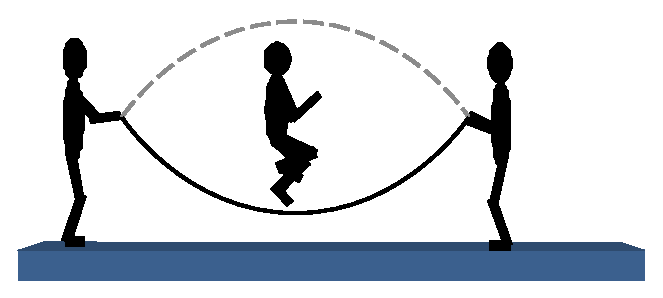
\includegraphics[natheight=3.749800in,natwidth=5.000400in,height=0.9262in,width=1.2306in]{Lab6_figs/JumpRope1stHar.eps}
\end{center}
This standing wave had a part that went up and down in the middle and two
parts that did not move much on each end (called nodes). But if you had a
bored kid, you might have seen a standing wave that looks like this.%
\begin{center}
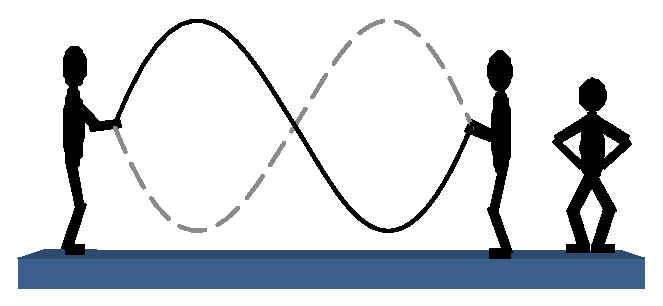
\includegraphics[natheight=3.749800in,natwidth=5.000400in,height=0.9446in,width=1.256in]{Lab6_figs/JumpRope2ndHar.eps}
\end{center}
This is not so good for jumping, but makes an interesting picture. The part in
the middle that does not seem to be moving is called a node. Really there are
also nodes on each end of the rope as well. So altogether there are three
nodes in this picture. We can make standing waves that have many nodes. If you
try this with a jump rope, you will find that the more nodes you have, the
faster you have to shake your end of the rope. Another way to say this is that
the frequency of your wave you are making must increase with the number of
nodes. This is part of today's model.

In the setup on your table, ring stands are holding strings, and there is an
oscillator on one end that has a frequency control box. The other end has a
pulley and a hanging mass to provide tension on the string.%
\begin{center}
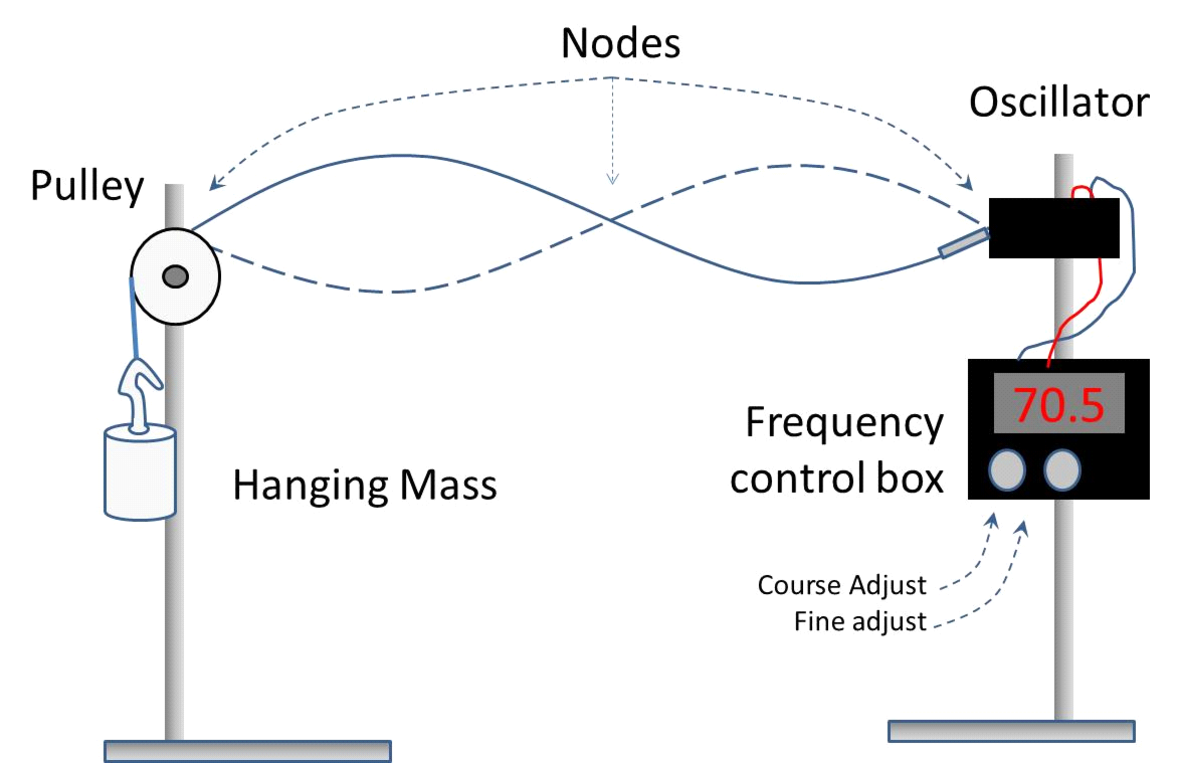
\includegraphics[natheight=1.907800in,natwidth=2.949000in,height=1.5451in,width=2.3753in]{Lab6_figs/StandingWaveonString.png}
\end{center}

Experimentally we find that not all frequencies will make standing waves. So
our model includes the idea that only some frequencies produce standing waves.
Our model also includes the idea that the weight of the string will change
which frequency will make a standing wave. If you play a stringed instrument,
you may have noticed that some strings are thicker than others. Thicker
strings have different standing wave frequencies than thinner strings. If you
study this model (some of you will in PH123), you can derive an equation that
tells which frequencies will work%
\begin{equation}
f=\frac{n}{2L}\sqrt{\frac{Mg}{\mu}}\label{tolinearize}
\end{equation}
where $n$ is an integer ($n=1,2,3\ldots$). This integer for strings is the
number of nodes minus one $n=n_{nodes}-1$. So you can form a standing wave,
then count the places that don't seem to move (remember the ends!) and
subtract one to find $n.$ The frequency that creates the standing wave should
be a function of $n.$ \textbf{Our model tells us that if we know }%
$n,$\textbf{\ we should be able to predict the frequency}. You will find that
for each way you can make a standing wave, a small range of frequencies will
make the standing wave, not just one, single frequency. But the frequency that
produces the largest standing wave is the one we want (biggest amplitude--or
the one for which the wave looks bigger) . That was the $f$ that was included
in forming our model equation. Of course there are other variables in our
equation, so we should find out what they are.

The quantity, $\mu,$ is the linear mass density. It is defined as mass of the
string divided by the length of the string. So $\mu$ tells us how massive the
string is.

The quantity, $L$ is the length of the string that is participating in the
waving, $g=9.8004\unit{m}/\unit{s}^2$ is the acceleration due to gravity, and $M$ is the hanging mass tied to
the end of the string beyond the pulley.

One way we could verify our model equation is to use it to predict one of the
input values. Let's use $\mu$. \textbf{The idea is to use our model equation
to somehow find }$\mu$\textbf{\ and then measure }$\mu$\textbf{\ to see if the
model equation prediction is good.}

It might be tempting to just solve the above equation for $\mu$ and report the
answer from one measurement. And of course that will work. But I want to see if you can use some of the things we learned.

We learned earlier that we can take more than one measurement, and use those
measurements together with a curve fit to solve for a fit parameter. I\ want
you to do this. The quantity $\mu$ should be in one of the fit parameters.
Then you can solve for $\mu$ using the fit parameter given by your python
linear fit code. This is a more robust way to find $\mu,$ and it is the way I want you to proceed (Even
if you solve for $\mu$ several times and take a mean and standard
deviation--it will work and it is a good experimental technique--but I want to
see if you can find and use your linear least squares code, so using your code
gives the most points).

You may have to adjust the amplitude knob on the frequency controller for some
frequencies to keep the apparatus from shaking itself apart. The frequency
controller has a fine and a course frequency adjust knob, and a digital
frequency display.

\section{Assignment}

As a group design an experiment to test the model. Your design should
include the steps from lab 5.

\begin{enumerate}
\item Identify the system to be examined. Identify the inputs and
outputs. Describe your system in your lab notebook.

\item Identify the model to be tested. Express the model in terms of
an equation representing a prediction of the measurement you will make. Record
this in your lab notebook. (If you have not solved this problem in your PH121
class yet, call me over and we will go through it together).

\item Plan how you will know if you are successful in your experiment.
Plan graphs or other reporting devices. Record this in your lab notebook. For
today's lab, I will provide the frequency control box, oscillator, rope, and pulleys. If you need
other equipment, ask.

\item Rectify your equation if needed. Record this in your lab
notebook.

\item Choose ranges of the variables. Record this in your lab
notebook.

\item Plan the experimental procedure. Record this in your lab
notebook.

\item Perform the experiment. Record this in your lab notebook. Go
through all the steps of performing an experiment. End with a conclusion that
clearly states whether your experiment supported the model, falsified the
model, or, if neither was possible, try to explain why.
\end{enumerate}



\end{document}
%\documentclass[twoside,11pt,ShortChapTitles]{BYUTextbook}

\usepackage{soul}
\renewcommand{\vec}[1]{\ensuremath{\mathbf{#1}}}
\usepackage{siunitx}
\sisetup{round-mode = figures,
  round-precision = 3, scientific-notation=true}
  \usepackage{marginfix}

\usepackage{mathtools}

\usepackage{listings}

\usepackage{color}

\definecolor{dkgreen}{rgb}{0,0.6,0}
\definecolor{gray}{rgb}{0.5,0.5,0.5}
\definecolor{mauve}{rgb}{0.58,0,0.82}

\lstset{frame=tb,
  language=Python,
  aboveskip=3mm,
  belowskip=3mm,
  showstringspaces=false,
  columns=flexible,
  basicstyle={\small\ttfamily},
  numbers=none,
  numberstyle=\tiny\color{gray},
  keywordstyle=\color{blue},
  commentstyle=\color{dkgreen},
  stringstyle=\color{mauve},
  breaklines=true,
  breakatwhitespace=true,
  tabsize=3, upquote=true}

\lstMakeShortInline[columns=fixed]|
\setcounter{chapter}{6}

\begin{document}



\chapter[Numerical modeling I]{Numerical modeling of Projectile motion}


\section{Assignment}

{\small Because we are learning a major new skill. we will take three weeks to
complete the experiment we are starting today. This will affect your lab
notebook. Complete each part of the lab each week in an organized fashion in
your lab notebook. Make graceful end-of-class entries so you can start up
again the following week. As always, part of the grade will be based on
neatness and organization!}

\begin{enumerate}
\item {\small Create a Python script that will numerically model the motion of
a spherical projectile shot straight up and then falling back down using
Euler's method. Assume there is no air resistance. As input quantities you
should provide the following:}

\begin{itemize}
\item {\small The initial }$y${\small \ position of the projectile } $y=70.00${\small \ meters}

\item {\small The initial speed of the projectile. }$30.0 \operatorname{m} / \operatorname{s} $

\item {\small The time step size.}$0.1${\small \ seconds}

\item {\small The acceleration due to gravity }$9.8 \operatorname{m} / \operatorname{s} ^{2}$
\end{itemize}

{\small Make these quantities variables so you can easily change values and
recalculate. The program in the precious section will walk you through this part. Save your script and record where you saved it.
Include a scatter plot of }${\small y}${\small \ vs }${\small t}${\small \ in
your lab notebook.}

\item {\small Copy and then modify your Python script to numerically model the
motion of a spherical projectile being launched from a cannon using Euler's
method. As input quantities you should add the following (Make these
quantities variables so you can easily change values and recalculate):}

\begin{itemize}
\item {\small The initial }$x${\small \ position of the projectile }$x=0.00$

\item {\small The launch angle for the projectile (measured from the positive
}$x${\small \ axis) }$45${\small \ degrees Include a plot of }$y${\small \ vs
}$x${\small \ in your lab notebook. Save your script and record where you
saved it.}
\end{itemize}

\item {\small Copy and modify your script to include air resistance. Air
resistance will add a new resistive force that is proportional to the square
of the projectile's velocity, i.e. } \[
F_{R}=\frac{1}{2}D\rho Av^{2}
\]
{\small where }$D${\small \ is the drag coefficient, }$\rho${\small \ is the
density of the air, }$A${\small \ is the cross-sectional area of the
projectile presented to the air (in our case }$A=\pi r^{2}${\small ), and }$v
${\small \ is the speed. The force is directed opposite the velocity of the
projectile. You will need components of this force. You should convince
yourself that } \begin{align*}
F_{R_{x}}  & =-\frac{1}{2}D\rho Av\left(  n\right)  v_{x}\left(  n\right) \\
F_{R_{y}}  & =-\frac{1}{2}D\rho Av\left(  n\right)  v_{y}\left(  n\right)
\end{align*}
{\small where } \[
v\left(  n\right)  =\sqrt{\left(  v_{x}\left(  n\right)  \right)  ^{2}+\left(
v_{y}\left(  n\right)  \right)  ^{2}}
\]
{\small and }$v_{x}\left(  n\right)  ${\small \ and }$v_{y}\left(  n\right)
${\small \ are the components of the velocity. This form of the components of
the resistive force avoids having to calculate the angle at each of our Euler
steps. As input quantities you should provide the following (Make these
quantities variables so you can easily change values and recalculate):}

\begin{itemize}
\item {\small The mass of the projectile:}
$0.020 \operatorname{kg} $

\item {\small The radius of the projectile:}
$0.02${\small \ meters}

\item {\small The drag coefficient for the projectile:}
$0.2$

\item {\small The density of the air the projectile travels through:}
$1.23 \operatorname{kg} / \operatorname{m} ^{3}$
\end{itemize}

\item {\small Include a scatter plot of your }$x${\small \ and } $y${\small \ positions for each time step in your lab notebook}
\end{enumerate}




\end{document}

\documentclass[twoside,11pt,ShortChapTitles]{BYUTextbook}

\usepackage{soul}
\renewcommand{\vec}[1]{\ensuremath{\mathbf{#1}}}
\usepackage{siunitx}
\sisetup{round-mode = figures,
  round-precision = 3, scientific-notation=true}
  \usepackage{marginfix}

\usepackage{mathtools}






\setcounter{chapter}{8}

\begin{document}
\chapter[Numerical Modeling II]{Numerical Modeling of a Mass-Spring System}
\section{Assignment}

{\small Complete this lab as a group and record your experience in an
organized fashion in your lab notebook. Part of the grade will be based on
neatness and organization!}

\begin{enumerate}
\item Copy, then modify your one dimensional Euler code and then
modify it to numerically model the motion of a mass-spring system with a
mass of 200.0 grams, a spring constant of 0.500 N/m, an initial displacement
from equilibrium of 15.0 cm, and an initial velocity of zero. Use a time
step of 0.01 seconds, and simulate the motion for a total of 20 seconds.
Graph your results, and comment.

\item  Repeat problem 1, but this time using a damped oscillator.
Damping is a resistive force that is opposite the direction the mass is
traveling. The resistive force has the form $F_{R}\left( n+1\right)
=bv\left( n\right) $ where$v\left( n\right) $ \ is the
mass speed and b is a constant that tells how much resistance the system has. In your modeling, use $b=0.05$  kg/s.

\item  Investigate what happens with each of the above modeling
scenarios when you increase or decrease the time step.

\item If there is time, try different masses, spring constants,
damping coefficients, and so on.

\end{enumerate}






\end{document}

\end{document}
